% Master article draft using the shared bibliography database OpenEcon_refs.bib.
\documentclass[11pt]{article}
\usepackage[utf8]{inputenc}
\usepackage[T1]{fontenc}
\usepackage{lmodern}
\usepackage[margin=1in]{geometry}
\usepackage{setspace}
\usepackage{amsmath,amssymb}
\usepackage{booktabs}
\usepackage{graphicx}
\usepackage{float}
\usepackage[section]{placeins}
\usepackage{array}
\usepackage{tabularx}
\usepackage{caption}
\usepackage{hyperref}
\usepackage{enumitem}
\usepackage{xcolor}
\usepackage{longtable}
\usepackage{multirow}
\usepackage{fancyvrb}
\usepackage[authoryear]{natbib}
\graphicspath{{photo/}}

\onehalfspacing
\setcounter{topnumber}{5}
\setcounter{bottomnumber}{5}
\setcounter{totalnumber}{8}
\renewcommand{\topfraction}{0.90}
\renewcommand{\bottomfraction}{0.85}
\renewcommand{\textfraction}{0.08}
\renewcommand{\floatpagefraction}{0.85}
\hypersetup{
    colorlinks=true,
    linkcolor=blue,
    citecolor=blue,
    urlcolor=blue
}

\title{\textbf{Are Economists Open to AI? \\ Text as Data as Survey on Professional Sentiment and Academic Research Trends}\thanks{{\footnotesize We appreciate the comments of Manuel L\'{o}pez Mart\'{i}n de Blas, Carlo Chiarella, John Coah, Eric Duca, Pablo Garc\'{i}a Est\'{e}vez, Juan Pedro Gomez, Pedro Alberto Chauffaille Saffi, Sergio Javier Garc\'{i}a Saiz, Iv\'{a}n Blanco S\'{a}nchez, Salom\'{o}n Garc\'{i}a Villegas and seminar participants at CUNEF university for generous conversations, careful suggestions, and encouragement at different stages of this project. Their comments helped sharpen the paper's framing and exposition. All remaining errors are our own.}}}

\author{
    Yi Wang\thanks{Renmin University of China. Email: \href{mailto:wy\_139@ruc.edu.cn}{wy\_139@ruc.edu.cn}}
    \and
    Lei Ge\thanks{Renmin University of China. Email: \href{mailto:gelei@ruc.edu.cn}{gelei@ruc.edu.cn}}
}

\date{\today}

\newcommand{\casepair}[2]{\begin{minipage}[t]{\linewidth}\vspace{0pt}\begin{itemize}[leftmargin=1.2em,noitemsep,topsep=0pt]\item #1\item #2\end{itemize}\end{minipage}}

\begin{document}

\maketitle

\begin{abstract}
\noindent Traditional surveys are costly, hard to reconstruct retrospectively, and vulnerable to self-presentation bias. Raw internet text is abundant but noisy, weakly structured, and platform-selected. We introduce TaDaS (Text as Data as Survey), a framework that converts naturally occurring text into survey-like evidence by linking a question corpus to an answer corpus through cross-dataset semantic retrieval. TaDaS first screens a reference question corpus to construct focal and comparable semantic neighborhoods. It then maps unstructured observations from an answer corpus onto these neighborhoods and scores the attitudes expressed in the resulting discourse. We apply the framework to economists' reactions to AI by linking 1.3 million research-related posts from Economics Job Market Rumors with 53,585 elite economics and finance publications. Publication-side topics define the research frontier; forum-side replies reveal professional sentiment along six dimensions: openness, negativity, toxicity, arrogance, curiosity, and confusion. AI-related discussion is less open and more negative in cross-section. In the preferred difference-in-difference-in-differences design, however, stronger publication-side AI visibility is associated with greater openness and curiosity and with lower negative tone, poisonousness, arrogance, and confusion, even after adding a post-2023 AI-wave indicator, alternative topic benchmarks, trend controls, high-versus-low AI-exposure heterogeneity, and saturated all-topic trend controls. The findings show how TaDaS can recover scalable, retrospective, and non-reactive measures of professional sentiment from existing text archives.
\end{abstract}

\vspace{1em}
\noindent \textbf{Keywords:} Artificial Intelligence, Text as Data as Survey, Professional Sentiment, Semantic Retrieval, Academic Research Trends, EJMR \\
\noindent \textbf{JEL Classification:} A11, C81, J24, O33

\clearpage

\section{Introduction}

Measuring attitudes is usually a survey problem. Researchers define questions, recruit respondents, and compare answers across people or time. This design remains powerful, but it is costly, slow to update, hard to reconstruct retrospectively, and vulnerable to response bias when respondents know the question is sensitive. The expansion of internet text creates a different possibility. Large archives of posts, comments, publications, reviews, and institutional records already contain traces of opinion, disagreement, curiosity, and resistance. Yet raw text is not a survey. It is noisy, platform-selected, weakly organized around researcher-defined questions, and difficult to convert into comparable attitude measures.

This paper introduces TaDaS (Text as Data as Survey), a framework for turning naturally occurring text into survey-like evidence. The core idea is double efficient information extraction. The first efficiency is on the question side: TaDaS extracts questions from a question corpus by screening the raw text into focal semantic neighborhoods and nearby comparison neighborhoods. The second efficiency is on the answer side: conditional on those efficiently extracted questions, TaDaS extracts survey-like opinions from a large unstructured corpus by mapping observations to a labeled answer corpus and scoring the relevant responses. In this sense, TaDaS is not simply text classification or sentiment analysis. It is a measurement architecture that makes unstructured text behave more like repeated survey evidence.

We apply TaDaS to a concrete question: are economists open to artificial intelligence (AI)? This setting is useful because direct survey responses may be filtered by professional status concerns and because retrospective survey data on fast-moving AI adoption are scarce. The application links two databases: Economics Job Market Rumors (EJMR), which provides naturally occurring professional discourse, and 53,585 elite economics and finance publications, which provide a labeled publication-side answer corpus. The two corpora are embedded in a shared semantic space, allowing the analysis to observe AI-related professional discussion and to ask whether its tone changes as AI becomes more visible in elite journals.

The application illustrates what TaDaS adds. Instead of asking economists directly whether they are open to AI, the framework observes how they argue, dismiss, defend, and engage when AI-related issues arise in professional conversation. Each reply is scored along six attitude dimensions: openness, negativity, toxicity, arrogance, curiosity, and confusion. The resulting evidence shows a two-sided pattern. In the static cross section, AI-related discussion is less open and more negative. In the preferred DDD design, stronger publication-side AI presence is associated with a favorable six-dimensional shift, and that pattern survives when the paper models the post-2023 AI wave explicitly. The substantive interpretation is descriptive: AI enters professional discourse under tension, and that tension is lower in periods when AI is more visible in the publication frontier.

The remainder of the paper proceeds as follows. Section \ref{sec:tadas} introduces the TaDaS framework. Section \ref{sec:literature} situates the paper in the relevant literatures. Section \ref{sec:data} describes the application data, topic-mapping procedure, and sentiment-measurement workflow. Section \ref{sec:model} presents the model, the main results, and their interpretation. Section \ref{sec:robustness} discusses robustness. Section \ref{sec:conclusion} draws the paper's main conclusions and outlines future directions.

\section{Text as Data as Survey}
\label{sec:tadas}

\subsection{Traditional Surveys and Internet Text}

Conventional surveys remain the natural benchmark for measuring attitudes because they impose a common question instrument on a known respondent population. Survey methodology also provides the cleanest vocabulary for sampling, question design, measurement error, and respondent behavior \citep{groves2009}. These strengths are precisely what make surveys difficult to replace. At the same time, they create practical constraints. Surveys are costly and time consuming to repeat across topics, years, and professional groups; they are difficult to reconstruct retrospectively once a new question becomes important; and they may elicit strategically moderated responses when the subject is status-laden or professionally sensitive \citep{bertrand2001,tourangeau2007}.

Internet text addresses some of these constraints by supplying large archives of naturally occurring language. Posts, comments, publications, reviews, firm disclosures, policy documents, and other written traces are often inexpensive to reuse and can be analyzed retrospectively \citep{gentzkow2019}. However, raw text is not survey evidence by itself. It usually lacks a researcher-defined question structure, contains large amounts of irrelevant material, reflects platform-specific selection, and stores useful information in a high-dimensional and weakly organized form. Automated text analysis therefore requires a measurement design that specifies which texts are being treated as questions, which texts supply the answer space, and how unstructured language becomes comparable variables \citep{grimmer2013}.

\subsection{The TaDaS Framework}

TaDaS is a measurement framework for converting naturally occurring text into survey-like evidence. It is designed for settings in which the researcher observes large text archives but does not observe a pre-fielded survey instrument. The framework separates the measurement problem into two linked corpora. The question corpus is the text environment in which the empirical question is posed and where attitudes, reactions, or outcomes are ultimately measured. The answer corpus is a labeled or labelable body of text that supplies the semantic coordinate system used to organize those reactions. The two corpora need not share users, authors, institutions, or identifiers; they only need to be embedded in a common semantic space.

The first component is efficient question extraction. Naturally occurring text does not arrive as a clean questionnaire: many observations are outside the researcher's object of interest, and many relevant observations are short, fragmented, or only partially informative. TaDaS therefore screens the question corpus before measurement. In this paper, the screen uses hierarchical density-based clustering, implemented through HDBSCAN, to retain focal semantic neighborhoods and nearby comparison neighborhoods. This step follows a common-support logic: focal observations should be compared with semantically adjacent observations, rather than with the entire raw archive. The screening step turns the raw question corpus into an empirical question set with local comparison structure. It also reduces measurement error by limiting the accumulation of sparsity-induced noise from weakly informative text. Appendix \ref{app:tadas_sample_screening} gives the formal screening rule.

The second component is efficient answer extraction. The answer corpus supplies the semantic categories relative to which the screened question-corpus observations are interpreted. Operationally, the answer corpus is embedded, clustered into substantive topics, and summarized by topic centers. Each screened observation from the question corpus is then projected onto these answer-corpus topic centers through cosine similarity in the shared embedding space. The output is a vector of continuous topic-exposure measures rather than a single hard topic label. A post can therefore be close to AI, Gender Economics, or Platform Economics by degree, which is closer to how survey questions can allow graded responses or multiple relevant dimensions. Appendix \ref{app:tadas_method} gives the formal projection representation.

The third component is attitude or outcome scoring. Once the question-corpus observations have been screened and mapped to answer-corpus topic directions, the researcher can measure the response attached to each question. In this application, an instruction-following decoder scores reply-level attitudes along several dimensions \citep{gilardi2023,ziems2024}. The decoder is not the defining feature of TaDaS. It is one possible scoring instrument used after the corpus-linking architecture has defined the question set and the answer space.

In the present paper, EJMR is the question corpus in which professional attitudes are observed, and elite-journal publications are the answer corpus that defines the research frontier. Publications supply labeled research-topic directions; EJMR supplies the professional discourse in which reactions to those directions are measured. The resulting variables are survey-like in the limited but useful sense that they convert naturally occurring text into repeated, labeled, comparable measures of topic exposure and attitude.

\begin{figure}[H]
    \centering
    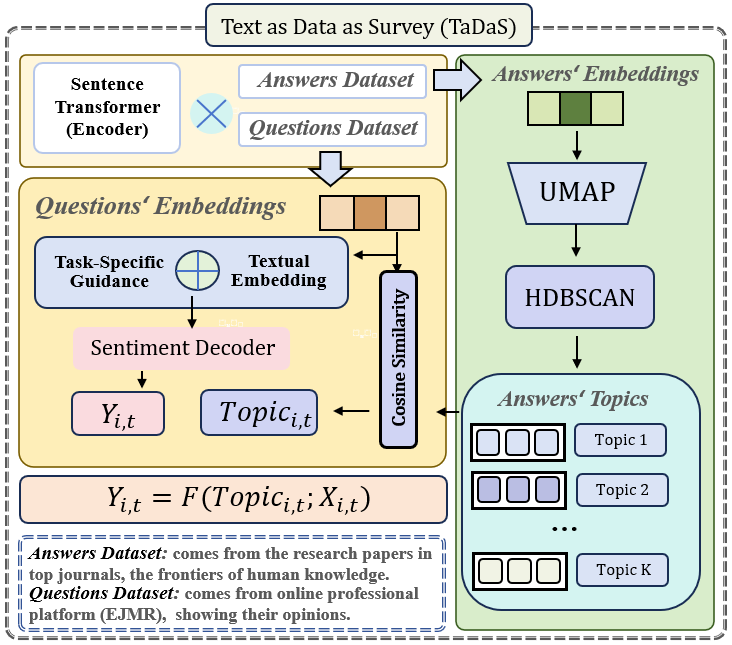
\includegraphics[width=0.7\textwidth]{workflow2.png}
    \caption{Text-as-Data Workflow Linking Publications and Forum Discussions}
    \label{fig:workflow}
\end{figure}

Figure \ref{fig:workflow} illustrates the architecture. A traditional survey design begins with a questionnaire and a sampling frame. A standard text-as-data design often remains within one corpus and measures topics or sentiment inside that corpus alone. TaDaS instead separates question formation, answer-space construction, and response scoring. The result is not a substitute for identification or validation. It is a measurement architecture that expands the set of survey-like questions researchers can ask using existing professional text.

\subsection{Advantages of TaDaS}

TaDaS is useful because it gives unstructured text a survey-like structure while preserving the scale, context, and retrospective coverage that make text archives valuable.

\textbf{Behavioral expression in context.} Compared with conventional surveys, TaDaS can capture attitudes as they are expressed in ordinary communication rather than only in direct elicitation. This is especially useful for sensitive professional topics, where respondents may soften disagreement, hostility, or status concerns in formal survey language. Compared with raw internet text, TaDaS imposes a semantic question frame and a disciplined comparison sample, making the recovered attitudes more interpretable.

\textbf{Low marginal cost of repeated measurement.} Once relevant text exists, the TaDaS workflow can turn large archives into structured attitude measures without fielding a new questionnaire for every topic, year, or respondent group. It therefore lowers the marginal cost of repeated survey-like measurement while still allowing the researcher to validate the scoring procedure.

\textbf{Flexible updating.} TaDaS can be rerun when new text arrives, when the answer-corpus topic system changes, or when researchers want to ask new questions of an existing archive. This makes it more flexible than many traditional surveys, whose question wording and sample frame are fixed at the time of fielding.

\textbf{Common-support sample discipline.} The question-corpus screen keeps focal topic neighborhoods together with nearby but not identical comparison neighborhoods. This matching-spirit design avoids comparing focal discussion to distant background conversation and reduces noise from short or weakly informative text.

\textbf{Cross-corpus portability.} TaDaS can connect corpora that cannot be merged through conventional identifiers. In this paper, publication text defines a semantic coordinate system for the research frontier, while EJMR text is measured relative to that system. The same logic could link professional forums to patents, policy documents, grants, product reviews, support tickets, or other labeled text databases.

\section{Related Literature}
\label{sec:literature}

\subsection{Semantic Representation, Topic Mapping, and Cross-Corpus Retrieval}

The measurement strategy builds on a topic-modeling tradition that treats large text collections as structured empirical objects. \citet{blei2003} introduced latent Dirichlet allocation as a probabilistic way to recover interpretable topics from high-dimensional word counts, and \citet{roberts2014} extended topic modeling toward open-ended survey responses and document-level covariates. This line of work matters for the present paper because it shows how text can be converted from raw language into a lower-dimensional empirical representation rather than read only as individual documents.

Recent embedding methods shift the measurement problem from word co-occurrence to semantic proximity. \citet{reimers2019} show that sentence-transformer representations can make semantic similarity practical at scale, while transformer models such as \citet{vaswani2017}, \citet{brown2020}, and \citet{ouyang2022} provide the broader language-modeling foundation for modern representation learning. The paper's topic construction also draws on dimensionality reduction and density-based clustering tools, especially UMAP \citep{mcinnes2018umap}, HDBSCAN \citep{campello2013hdbscan,mcinnes2017hdbscan}, and BERTopic-style c-TF-IDF topic summaries \citep{grootendorst2022bertopic}.

The cross-corpus use of semantic structure also connects to studies that use topic movement to measure institutional or intellectual change. \citet{locatelli2023} use topic shifts to study politicization in public communication, \citet{goldsmithpinkham2024} traces the credibility revolution across fields, and \citet{bello2025} uses research similarity to study gendered academic patterns. \citet{pramanick2026} similarly studies how large language models reshape scholarly landscapes across fields. This paper follows these studies in treating semantic movement as substantively meaningful, but it uses publication-side topic structure to organize forum-side professional reactions.

\subsection{Text as Data in Social Science}

Text as data has become a central empirical approach in economics and related social sciences. \citet{gentzkow2019} provide a broad overview of text as data in economics, emphasizing both the promise of scalable measurement and the importance of validation. \citet{grimmer2013} similarly stress that automated text analysis requires explicit design choices rather than mechanical extraction. \citet{hassan2025} extend this agenda by showing how computational linguistics can recover economic information from corporate-generated text, including earnings calls, patents, and job postings.

Several influential applications show how text can produce economic variables that would otherwise be difficult to observe. \citet{baker2016} construct an economic policy uncertainty index from newspaper text, while \citet{loughran2011} show that finance-specific dictionaries matter for interpreting 10-K language. \citet{hoberg2016} use firm product descriptions to build text-based industry networks, and \citet{xiu2024} use business news to study business cycles. These papers are useful benchmarks because they show that text can measure latent economic conditions, competitive environments, and aggregate narratives.

More recent work uses richer models to extract signals from financial and organizational text. \citet{fan2024} study misinformation in financial markets, \citet{siano2025} uses LLM methods to capture the news in earnings disclosures, and \citet{li2024} develops a structural topic and sentiment-discourse model for text analysis. \citet{lin2024} construct textual factors for scalable and interpretable analysis of unstructured information. Relative to these single-corpus applications, this paper links two corpora: publications define the research frontier, while EJMR replies supply the professional attitudes to be measured.

\subsection{Anonymous Professional Discourse and EJMR}

The paper also relates to research on anonymous professional discourse, especially EJMR. \citet{wu2018} shows that gendered language on EJMR reflects broader asymmetries in the economics profession. \citet{ederer2025} study attention and abuse in anonymous economics discourse and show why EJMR is useful for observing professional behavior that may be muted in less anonymous settings. These EJMR studies motivate the use of anonymous forum text as evidence about hierarchy, exclusion, and professional conflict.

Work outside economics helps explain why anonymous online communication can differ from formal survey responses or public professional statements. \citet{suler2004} describes the online disinhibition effect, and \citet{cheng2017} show that antisocial behavior in online discussions depends partly on context and prior interaction. \citet{alberti2024} documents toxic communication around the accounting academic job market, while \citet{flores2023} distinguishes passive and proactive online behavior modes. These studies suggest that online professional forums are noisy but structured settings in which tone, engagement, and conflict can be measured empirically.

The present paper builds on this literature by treating EJMR neither as a representative survey nor as pure noise. Following \citet{wu2018} and \citet{ederer2025}, the forum is useful because it records professional status talk, gatekeeping, and abuse at scale. Following \citet{suler2004} and \citet{cheng2017}, its anonymity also requires caution because the same environment that reveals low-filter reactions can amplify hostility. This motivates the paper's focus on repeated discourse patterns rather than claims about the average private belief of all economists.

\subsection{AI Adoption, Work, and Scientific Production}

Finally, the empirical question connects to work on AI, automation, and the organization of production. \citet{autor2015} frames automation as a task-level process that changes the boundary between human and machine work. \citet{felten2021} develop measures of occupational, industry, and geographic exposure to AI, and \citet{acemoglu2022} study AI exposure through online vacancies. \citet{eloundou2023} extend the exposure approach to large language models and characterize the tasks most affected by LLM capabilities.

Evidence on realized AI use shows that the technology can change productivity and work organization. \citet{noy2023} provide experimental evidence on the productivity effects of generative AI in writing tasks, and \citet{brynjolfsson2025} provide field evidence on generative AI at work. \citet{kanazawa2025} study AI, skill, and productivity among taxi drivers, showing that AI can complement workers in field settings. These papers clarify why AI may be attractive as a tool while also changing the value of existing skills.

The scientific-production literature is especially relevant because the paper studies economists' reactions to AI inside an academic profession. \citet{hao2025} argue that AI tools can expand scientists' impact while narrowing scientific focus, and \citet{pramanick2026} documents the influence of large language models across academic fields beyond computer science. This paper complements these studies by measuring professional discussion around AI as AI becomes more visible in elite economics and finance journals.

\subsection{What This Paper Adds}

Relative to these literatures, the paper contributes by connecting three objects that are usually studied separately: text-based measurement, anonymous professional discourse, and the professional diffusion of AI.

First, the paper extends the text-as-data tradition toward a \textit{text as data as survey} framework. Existing work has shown that text can recover economically meaningful information from policy documents, firms, news, and research corpora. This paper uses that insight for a different measurement problem: recovering structured attitudes from naturally occurring professional conversation. The key move is not simply to classify text, but to turn high-volume, unprompted discourse into survey-equivalent attitude measures that can be linked to changes in the research frontier. This is especially useful when direct surveys may be costly, infrequent, or vulnerable to self-presentation.

Second, the paper reframes EJMR as a source of professional sentiment rather than only as an object of concern. Prior EJMR research documents bias, abuse, and hierarchy in anonymous professional communication. This paper builds on that evidence but uses the forum for a different purpose: to observe how economists react to a new research technology in a setting with low reputational filtering, repeated professional interaction, and visible gatekeeping. EJMR is therefore not treated as representative of all economists in a survey-sampling sense. Instead, it is used as a behavioral archive where disagreement, status anxiety, adaptation, and exclusion can be observed at scale.

Third, the paper links the AI-adoption literature to publication-side visibility in academic economics. Existing studies ask how AI affects labor demand, productivity, task exposure, and scientific work. This paper asks a complementary question: as AI becomes more visible in elite journals, does professional discussion of AI shift across multiple attitude dimensions? The encoder-decoder design makes that question empirically tractable. The encoder side maps publications and forum posts into a shared semantic topic space, while the decoder side converts replies into interpretable attitude dimensions. Taken together, these elements allow the paper to study not only whether economists talk about AI, but also how their reactions co-move with AI's presence in the publication frontier.

\section{Data}
\label{sec:data}

\subsection{Questions Corpus and Questions Topic Construction}

The questions (publication-side) corpus contains 53,585 papers drawn from elite economics and finance journals closely aligned with the ABS 4* tier. This corpus serves as the answer corpus in the TaDaS design because it provides a stable, labeled map of the recognized research frontier. Elite journals are useful for this purpose because they collect work that has passed through visible professional filters and therefore provide a disciplined source for constructing topic directions. This interpretation is consistent with classic accounts of scientific recognition and the diffusion of ideas through scholarly communities \citep{merton1968,bourdieu1975,crane1972}.

Each publication record contributes title and abstract text, which are used to recover a topic structure and calculate annual topic intensities. Each topic's annual intensity series is treated as a publication-side adoption proxy and named as the corresponding \texttt{XX\_Trend} variable. \texttt{AI\_Trend} is the adoption proxy for the AI topic and is the focal trend variable in this paper. AI is a useful focal case because it is both a research object and a research technology: it affects what economists study, but it also affects how they code, write, search, summarize, referee, and train students. As AI-related work appears more often in elite journals, this publication-side visibility may coincide with less treatment of AI as unserious, peripheral, or external to the discipline.

\begin{figure}[H]
    \centering
    \includegraphics[width=0.8\textwidth]{field_distribution.png}
    \caption{Field Distribution in the Publication Corpus}
    \label{fig:field_distribution}
\end{figure}

\begin{figure}[H]
    \centering
    \includegraphics[width=0.7\textwidth]{journal_distribution.png}
    \caption{Journal Distribution in the Publication Corpus}
    \label{fig:journal_distribution}
\end{figure}

Publication-side topic construction also relies on All-RoBERTa Large v1 (\texttt{all-roberta-large-v1}) \citep{liu2019roberta,reimers2019}. Titles and abstracts are embedded with this encoder and then grouped into a publication-side topic structure that can be tracked over time. In the current pipeline, the high-dimensional encoder vectors are first compressed with UMAP and then clustered with HDBSCAN, after which cluster-level keywords are recovered with class-based TF-IDF \citep{mcinnes2018umap,campello2013hdbscan,mcinnes2017hdbscan,grootendorst2022bertopic}. The publication data then yield annual topic-intensity series such as \texttt{AI\_Trend}, \texttt{Gender\_Economics\_Trend}, and \texttt{Platform\_Economics\_Trend}. These series are constructed in the same way: for each publication-side topic, the paper aggregates the topic's annual intensity in the elite-journal corpus and uses the resulting time series as that topic's adoption proxy. In operational terms, \texttt{AI\_Trend} is the AI-specific member of this family of \texttt{XX\_Trend} variables. Appendix Sections \ref{app:transformer_background} and \ref{app:topic_clusters} provide a formal explanation of the transformer background, the UMAP-HDBSCAN-c-TF-IDF pipeline, and the way topic similarity is computed from publication-side topic centers to EJMR-side text vectors.

\begin{figure}[H]
    \centering
    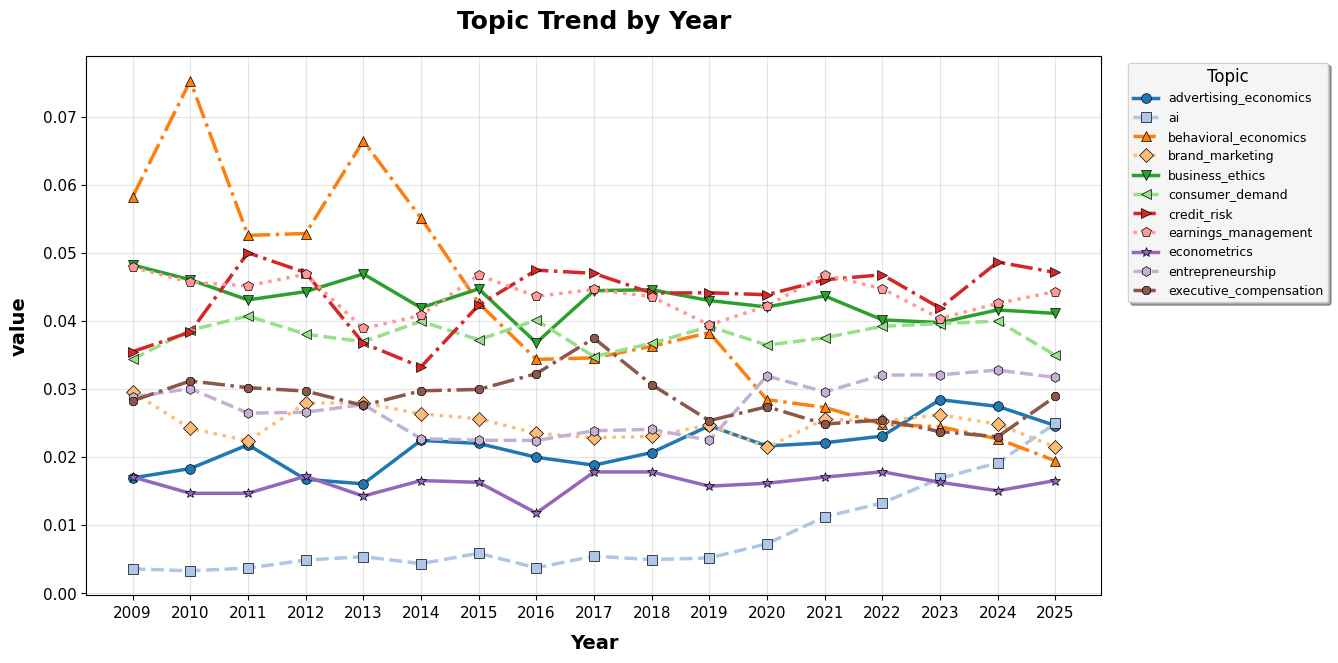
\includegraphics[width=0.96\textwidth]{Proxy_Trend.png}
    \caption{Illustrative Trends in Publication-Side Topic Proxies}
    \label{fig:proxy_trend}
\end{figure}

Figure \ref{fig:proxy_trend} reports selected annual publication-side topic series. \texttt{AI\_Trend} is the series for the AI topic, and additional publication-side topic proxy panels are reported in Appendix Figures \ref{fig:appendix_proxy_trend_2} and \ref{fig:appendix_proxy_trend_3}.

The current main specification is built on the ABS 4* journal sample and contains 32 publication-side research topics. These labels should be read as semantic summaries of publication clusters rather than as manually imposed fields. The resulting inventory covers AI, econometrics, health economics, family business, labor and wages, gender economics, personnel economics, public governance, firm strategy, behavioral economics, venture capital, entrepreneurship, supply chains, game theory, mergers and acquisitions, executive compensation, online reviews, platform economics, innovation and patents, international business, credit risk, business ethics, team productivity, advertising economics, retail pricing, racial inequality, intergenerational mobility, risk preferences, consumer demand, brand marketing, hedge funds, and earnings management.

To make the publication-side construction transparent, Table \ref{tab:paper_topic_keywords} reports the full topic inventory together with representative high-weight keywords, while Appendix Table \ref{tab:paper_topic_cases} reports illustrative paper titles associated with each topic. These materials clarify that the topic system is broad enough to cover multiple research domains beyond AI alone and that the topic labels are grounded in recognizable publication content rather than ad hoc naming choices.

\begingroup
\scriptsize
\setlength{\LTcapwidth}{\textwidth}
\begin{longtable}{p{0.18\textwidth}p{0.10\textwidth}p{0.62\textwidth}}
\caption{Publication-Side Topics and Representative Keywords}\label{tab:paper_topic_keywords}\\
\toprule
Topic & Papers & Representative keywords \\
\midrule
\endfirsthead
\toprule
Topic & Papers & Representative keywords \\
\midrule
\endhead
AI & 495 & artificial intelligence; intelligence ai; ai; human machine; machine learning \\
Econometrics & 618 & estimators; estimator; estimating; estimated; inference \\
Health Economics & 543 & patients; hospitals; hospital; health insurance; healthcare \\
Family Business & 458 & family firms; family firm; families; family; owned firms \\
Labor and Wages & 1,549 & wages; wage; minimum wage; unemployment; wage inequality \\
Gender Economics & 1,400 & gender diversity; gender bias; gender equality; gender gap; gender differences \\
Personnel Economics & 904 & human resource; human resources; hr; organizational performance; hrm research \\
Public Governance & 2,160 & administration research; bureaucracy; governance; bureaucracies; administration \\
Firm Strategy & 3,153 & organization studies; management research; strategy research; digital transformation; organization theory \\
Behavioral Economics & 2,183 & working memory; perceptual; visual; perception; memory \\
Venture Capital & 1,278 & venture capitalists; venture capital; investors; capital firms; startups \\
Entrepreneurship & 2,105 & entrepreneurship literature; entrepreneurship; entrepreneurial activity; entrepreneurial orientation; entrepreneurs \\
Supply Chain Economics & 741 & supply chains; value chain; supply chain; suppliers; supplier \\
Game Theory & 1,141 & nash equilibrium; payoffs; equilibrium outcome; cooperation; equilibria \\
Mergers and Acquisitions & 746 & mergers acquisitions; acquisitions; merger acquisition; acquisition; mergers \\
Executive Compensation & 1,826 & corporate governance; ceo compensation; ceo turnover; executive compensation; officers ceos \\
Online Reviews & 758 & product reviews; online reviews; reviews; sentiment; rating systems \\
Platform Economics & 768 & platform owners; digital platforms; digital platform; platforms; revenue sharing \\
Innovation and Patents & 2,661 & patents; patenting; innovation performance; patent; open innovation \\
International Business & 2,157 & multinational enterprises; international business; emerging markets; connected firms; multinationals \\
Credit Risk & 3,005 & borrowers; credit risk; lending; default risk; credit default \\
Business Ethics & 3,336 & ethical leadership; organizational justice; unethical behavior; justice perceptions; moral \\
Team Productivity & 1,287 & leadership; organizational citizenship; team performance; teamwork; group performance \\
Advertising Economics & 630 & advertisements; advertisement; ad; ads; consumer search \\
Retail Pricing & 1,165 & retailers; price competition; wholesale; dynamic pricing; inventory \\
Racial Inequality & 1,186 & racial disparities; police; blacks; officers; policing \\
Intergenerational Mobility & 1,896 & intergenerational mobility; income inequality; social mobility; educational attainment; low income \\
Risk Preferences & 3,926 & risk attitudes; ambiguity aversion; risk preferences; risk aversion; prospect theory \\
Consumer Demand & 1,802 & consumer psychology; purchase decisions; price discounts; discounts; discount \\
Brand Marketing & 3,661 & brands; consumers perceive; consumer psychology; purchase intentions; brand \\
Hedge Funds & 1,666 & hedge fund; hedge funds; fund managers; fund performance; mutual funds \\
Earnings Management & 2,381 & earnings forecasts; earnings management; earnings; forecasts; financial reporting \\
\bottomrule
\end{longtable}
\endgroup

\subsection{The Answers Corpus and Forum-Side Topic Mapping}

With the publication-side topic system defined, the forum-side corpus can be screened and mapped into the same semantic space. The Answers (forum-side) corpus comes from EJMR, an anonymous professional discussion environment that combines serious research discussion, labor-market anxiety, status signaling, methodological debate, and conflict. This mixture makes EJMR noisy, but it also makes it useful for TaDaS: the forum preserves weakly filtered professional reactions that would often be softened in a direct survey \citep{bertrand2001,tourangeau2007}.

\begin{figure}[H]
    \centering
    \includegraphics[width=0.82\textwidth]{EJMR_frontpage}
    \caption{EJMR as a Professional Discussion Environment}
    \label{fig:ejmr_frontpage}
\end{figure}

The broader raw EJMR archive contains 7,989,637 posts. The main EJMR analysis sample contains about 1,304,483 post-level observations from 2010 to 2024 after a research-oriented screening step. The motivating example in Table \ref{tab:motivating_quotes} shows why the forum is useful for measuring professional reactions to AI. The same thread contains both gatekeeping responses that defend existing training standards and open responses that treat generative AI, reinforcement learning, and NLP as part of the future skill set for economists.

\begin{table}[H]
    \centering
    \caption{An Example on EJMR of Economists' Opinions toward AI}
    \label{tab:motivating_quotes}
    \small
    \setlength{\tabcolsep}{6pt}
    \renewcommand{\arraystretch}{1.5}
    \begin{tabularx}{\textwidth}{@{}>{\raggedright\arraybackslash}X | >{\raggedright\arraybackslash}X@{}}
        \toprule
        \multicolumn{2}{@{}l}{\href{https://www.econjobrumors.com/topic/should-the-econ-grad-core-include-generative-ai-reinforcement-learning-nlp}{\textbf{Thread title}: Should the econ grad core include Generative AI, Reinforcement Learning, NLP? (2023)}} \\
        \midrule
        \textbf{Gatekeeping views} & \textbf{Open views} \\
        \midrule
        \textit{``Do you even know what reinforcement learning is?''} &
        \textit{``Seems like these are the future and econ hasn't changed since 1950.''} \\
        \midrule
        ``RL is basically approximate dynamic programming---a staple of the curriculum since the 80s.'' &
        ``To get hired in 2023 without an academic job, we're stuck taking Coursera and Udemy classes...'' \\
        \midrule
        ``Making it `core' means qualifying exams on ML, which is nonsense.'' &
        ``...this is after 5 years post-undergrad in Econ. It's time to adapt.'' \\
        \bottomrule
    \end{tabularx}
{\captionsetup{justification=raggedright,singlelinecheck=false}
\caption*{\footnotesize Notes: The table reports selected posts from the same EJMR thread. The left column illustrates gatekeeping responses that defend existing training standards or reject AI-related methods as inappropriate for the core curriculum. The right column illustrates open responses that frame generative AI, reinforcement learning, and NLP as part of the future skill set for economists.}}
\end{table}

EJMR also contains many topic areas that are far from research or professional academic activity. Alongside threads about methods, journals, research trends, and academic work, the forum contains everyday conversation about entertainment, food, exercise, cars, and other non-research subjects. The analysis sample therefore applies a research-oriented screening step before constructing forum-side topic exposure.

\begin{figure}[H]
    \centering
    \begin{minipage}[t]{0.31\textwidth}
        \centering
        \includegraphics[width=\linewidth]{2014_Case_EJMR_most_overated_cusine.png}
        \caption*{\footnotesize Food}
    \end{minipage}\hfill
    \begin{minipage}[t]{0.31\textwidth}
        \centering
        \includegraphics[width=\linewidth]{2016_Case_EJMR_How_much_do_you_exercise_in_a_week_and_what.png}
        \caption*{\footnotesize Exercise}
    \end{minipage}\hfill
    \begin{minipage}[t]{0.31\textwidth}
        \centering
        \includegraphics[width=\linewidth]{2021_Case_EJMR_best_new_cars.png}
        \caption*{\footnotesize Cars}
    \end{minipage}
    \caption{Examples of EJMR Threads Outside Research Discussion}
    \label{fig:ejmr_nonresearch_examples}
\end{figure}

Figure \ref{fig:ejmr_nonresearch_examples} makes the screening step concrete by showing ordinary forum conversations outside research discussion.

Operationally, EJMR texts are clustered in semantic space with HDBSCAN \citep{campello2013hdbscan,mcinnes2017hdbscan}. The procedure uses the HDBSCAN hierarchy to identify research-related topic clusters, retain their nearest local hierarchical neighbors, and exclude branches whose local hierarchy contains no neighboring research topic.

\begin{figure}[H]
    \centering
    \includegraphics[width=0.9\textwidth]{hierarchical_map.png}
    \caption{Illustrative EJMR Topic Hierarchy Used for Sample Screening}
    \label{fig:ejmr_hierarchical_map}
\end{figure}

Figure \ref{fig:ejmr_hierarchical_map} illustrates the logic. In the displayed hierarchy, the AI topic and the nearby \textit{ChatGPT} topic are retained because they sit in the local neighborhood of research-related discussion. By contrast, the \textit{movie} and \textit{star} topics below them are not retained because their local branch contains no neighboring research topic. Appendix Figure \ref{fig:ejmr_hierarchical_overview} reports the complete EJMR clustering hierarchy.

Forum-side topic exposure is measured by passing EJMR thread titles or post text through the same encoder used on the publication side and then mapping each forum observation to the publication-derived topic centers. The shared embedding model is All-RoBERTa Large v1 (\texttt{all-roberta-large-v1}), a sentence-transformer style encoder built on RoBERTa representations \citep{liu2019roberta,reimers2019}. Using the same encoder on both corpora ensures that forum-side topic exposure and publication-side topic centers are measured in a comparable vector space.

This mapping step produces post-level topic-exposure measures for AI and the other publication topics. The paper therefore identifies topic exposure semantically rather than through a narrow keyword list. A post can be close to the AI topic if its embedding is close to the AI topic center, even when the text uses related language such as machine learning, coding, automation, software tools, or changes in research skills.

\begin{figure}[H]
    \centering
    \includegraphics[width=0.88\textwidth]{EJMR_Topic_Distribution.png}
    \caption{Annual Topic Distribution in EJMR Discussions}
    \label{fig:ejmr_topic_distribution}
\end{figure}

Figure \ref{fig:ejmr_topic_distribution} reports the annual distribution used in the empirical analysis. The figure is descriptive and is shown before the regression results.

\subsection{Sentiment and Attitude Scoring}

The project uses a multidimensional scoring framework instead of a simple positive-negative polarity classification. The main post-level outcomes are openness, negative tone, poisonousness, arrogance, curiosity, and confusion.

The response scoring stage is carried out with the instruction-tuned decoder model Gemma 3 12B IT (\texttt{gemma-3-12b-it}) \citep{gemmateam2025}. This use of an instruction-following model as a structured text annotator is consistent with recent evidence that large language models can perform social-science annotation tasks at scale, while still requiring careful prompt design and validation \citep{gilardi2023,ziems2024}. The decoder is asked to return a vector of bounded attitude scores, with each component constrained to $[0,1]$, given a prompt post $Q_j$ and a reply $A_j$. The full prompt template used for scoring is reproduced in Appendix \ref{app:sentiment_prompt}.

As a simple face-validity check on the scoring prompt, Table \ref{tab:scoring_audit_cases} reports several illustrative reply-level cases. The examples show that the model-generated scores generally move in the same direction as ordinary human annotation intuition: information-seeking replies receive higher openness and curiosity, categorical dismissal receives higher negativity, alarmist replies receive low openness and high negative tone, and short jokes remain close to the neutral midpoint.

\begin{table}[H]
    \centering
    \caption{Illustrative Reply-Level Scoring Checks}
    \label{tab:scoring_audit_cases}
    \scriptsize
    \setlength{\tabcolsep}{3pt}
    \renewcommand{\arraystretch}{1.08}
    \begin{tabularx}{\textwidth}{p{0.24\textwidth} X p{0.19\textwidth} p{0.24\textwidth}}
        \toprule
        Thread Title & Reply excerpt & Scores & Human-intuition check \\
        \midrule
        Anyone using Haskell? &
        ``Any good books for using Haskell with econ/finance data?'' &
        Openness 0.8; curiosity 0.7; negative 0.3 &
        A direct request for recommendations is naturally read as open and curious, with little negative tone. \\
        Mining Causality: AI Assisted Search for Instrumental Variables &
        ``We propose using large language models (LLMs) to search for new IVs through narratives and counterfactual reasoning.'' &
        Openness 0.8; curiosity 0.7; negative 0.2 &
        The reply describes a concrete research use case and reads as constructive engagement rather than dismissal. \\
        AI systems can't create new knowledge, it just tells you what you already know &
        ``The current LLM paradigm can't create new knowledge. AlphaZero/MuZero can though...'' &
        Openness 0.8; curiosity 0.7; negative 0.2 &
        The reply disagrees with the premise but does so by reasoning through mechanisms, so high openness is intuitive. \\
        Reminder: ML and LLM are pseudo scientific &
        ``There is zero scientific evidence that machines can `think' or that large language models have anything to do with real language.'' &
        Openness 0.2; negative 0.8; poisonous 0.6 &
        The categorical language is strongly skeptical and dismissive, matching the high negative score. \\
        An Early Look at the Labor Market Impact Potential of Large Language Models &
        ``It's over for the middle class... Middle class jobs will vanish due to AI.'' &
        Openness 0.0; negative 1.0; curiosity 0.0 &
        The reply gives a closed and highly pessimistic forecast, so low openness and high negativity are natural. \\
        \bottomrule
    \end{tabularx}
{\captionsetup{justification=raggedright,singlelinecheck=false}
\caption*{\footnotesize Notes: The examples are drawn from audit cases of the reply-level scoring output. They are not used as separate regression evidence. They show that the scoring prompt produces attitude profiles that are close to ordinary annotation intuition across constructive, dismissive, alarmist, and neutral replies.}}
\end{table}

\subsection{Control Variables}

The regressions progressively introduce forum indicators, year fixed effects, and thread-title emotion controls.

The thread-title emotion controls are important because the tone of the original post can shape the tone of the response. A deliberately provocative question should not automatically be interpreted as evidence that the topic itself generates hostility.

The main text focuses on four progressive control combinations: year fixed effects only, year fixed effects plus forum indicators, year fixed effects plus thread-title emotion controls, and the full specification with both control families. The appendix reports the complete eight-column grid.

\subsection{Descriptive Statistics}

\begin{table}[H]
    \centering
    \caption{Main Sample Summary}
    \label{tab:sample_summary}
    \begin{tabular}{p{0.57\textwidth}r}
        \toprule
        Item & Count \\
        \midrule
        EJMR analysis sample & 1,304,483 \\
        Publication corpus & 53,585 \\
        Main topic system & $32$ topics \\
        Main EJMR sample period & $2010$--$2024$ \\
        \bottomrule
    \end{tabular}
\end{table}

The sample summary shows that the project is large along both margins: the professional corpus is large enough to support high-dimensional text measurement, and the publication corpus is broad enough to construct a time-varying research frontier.

\begin{center}
\scriptsize
\setlength{\tabcolsep}{4pt}
\begin{longtable}{lrrrrr}
\caption{Detailed Descriptive Statistics for Main Variables and Topic Exposures}\label{tab:descriptive_means}\\
\toprule
Variable & N & Mean & Std. Dev. & Min & Max \\
\midrule
\endfirsthead
\multicolumn{6}{l}{\tablename\ \thetable{} -- continued from previous page}\\
\toprule
Variable & N & Mean & Std. Dev. & Min & Max \\
\midrule
\endhead
\midrule
\multicolumn{6}{r}{Continued on next page}\\
\endfoot
\bottomrule
\endlastfoot
\addlinespace
\multicolumn{6}{l}{\textit{Core variables}} \\
year & 1304483 & 2018.2167 & 3.9236 & 2010.0000 & 2024.0000 \\
openness & 1304483 & 0.4556 & 0.2247 & 0.0000 & 1.0000 \\
negative & 1304483 & 0.5540 & 0.2353 & 0.0000 & 1.0000 \\
poisonous & 1304483 & 0.4878 & 0.2412 & 0.0000 & 1.0000 \\
arrogance & 1304483 & 0.5115 & 0.1885 & 0.0000 & 1.0000 \\
curiosity & 1304483 & 0.4082 & 0.2196 & 0.0000 & 1.0000 \\
confusion & 1304483 & 0.4325 & 0.1719 & 0.0000 & 1.0000 \\
Trend ai & 1304483 & 0.0086 & 0.0050 & 0.0033 & 0.0191 \\
\addlinespace
\multicolumn{6}{l}{\textit{Publication-side topic exposures}} \\
ai & 1304483 & 0.1068 & 0.1006 & -0.1747 & 0.6756 \\
econometrics & 1304483 & 0.1116 & 0.1056 & -0.1575 & 0.7293 \\
health economics & 1304483 & 0.0636 & 0.0774 & -0.1713 & 0.6961 \\
family business & 1304483 & 0.0625 & 0.0761 & -0.1623 & 0.6697 \\
labor wages & 1304483 & 0.0874 & 0.0962 & -0.1567 & 0.6965 \\
gender economics & 1304483 & 0.0887 & 0.0867 & -0.1831 & 0.6645 \\
personnel economics & 1304483 & 0.0576 & 0.0810 & -0.1880 & 0.6176 \\
public governance & 1304483 & 0.0758 & 0.0810 & -0.1711 & 0.5821 \\
firm strategy & 1304483 & 0.1131 & 0.1011 & -0.1644 & 0.6777 \\
behavioral economics & 1304483 & 0.1307 & 0.0805 & -0.1550 & 0.4953 \\
venture capital & 1304483 & 0.0876 & 0.0984 & -0.1653 & 0.7507 \\
entrepreneurship & 1304483 & 0.0724 & 0.0803 & -0.1615 & 0.7306 \\
supply chain economics & 1304483 & 0.0460 & 0.0817 & -0.1848 & 0.5419 \\
game theory & 1304483 & 0.0747 & 0.0915 & -0.1804 & 0.7145 \\
mergers acquisitions & 1304483 & 0.0725 & 0.0933 & -0.1765 & 0.7974 \\
executive compensation & 1304483 & 0.0781 & 0.0924 & -0.1916 & 0.7405 \\
online reviews & 1304483 & 0.0900 & 0.0849 & -0.1801 & 0.6071 \\
platform economics & 1304483 & 0.0809 & 0.0911 & -0.1628 & 0.7064 \\
innovation patents & 1304483 & 0.0833 & 0.0902 & -0.1900 & 0.7821 \\
international business & 1304483 & 0.0733 & 0.0889 & -0.1655 & 0.5930 \\
credit risk & 1304483 & 0.0755 & 0.0983 & -0.1772 & 0.6832 \\
business ethics & 1304483 & 0.0742 & 0.0853 & -0.1698 & 0.5989 \\
team productivity & 1304483 & 0.0531 & 0.0727 & -0.1847 & 0.6338 \\
advertising economics & 1304483 & 0.0821 & 0.0833 & -0.1590 & 0.6087 \\
retail pricing & 1304483 & 0.0545 & 0.0918 & -0.2004 & 0.6381 \\
racial inequality & 1304483 & 0.0894 & 0.0858 & -0.1742 & 0.6715 \\
intergenerational mobility & 1304483 & 0.1180 & 0.1020 & -0.1690 & 0.7300 \\
risk preferences & 1304483 & 0.1211 & 0.1037 & -0.1716 & 0.7197 \\
consumer demand & 1304483 & 0.0869 & 0.0934 & -0.1549 & 0.7267 \\
brand marketing & 1304483 & 0.0875 & 0.0826 & -0.1614 & 0.6964 \\
hedge funds & 1304483 & 0.0949 & 0.1102 & -0.1509 & 0.7277 \\
earnings management & 1304483 & 0.1098 & 0.1176 & -0.1889 & 0.7227 \\
\end{longtable}
\end{center}
{\captionsetup{justification=raggedright,singlelinecheck=false}
\noindent\footnotesize Notes: The table reports main sample moments for the attitude outcomes, AI\_Trend, and publication-side Topic\_Exposure measures used in the regression specifications.\normalsize}

\begin{center}
\scriptsize
\setlength{\tabcolsep}{4pt}
\begin{longtable}{lrrrrr}
\caption{Detailed Descriptive Statistics for Control Variables}\label{tab:descriptive_controls}\\
\toprule
Variable & N & Mean & Std. Dev. & Min & Max \\
\midrule
\endfirsthead
\multicolumn{6}{l}{\tablename\ \thetable{} -- continued from previous page}\\
\toprule
Variable & N & Mean & Std. Dev. & Min & Max \\
\midrule
\endhead
\midrule
\multicolumn{6}{r}{Continued on next page}\\
\endfoot
\bottomrule
\endlastfoot
\addlinespace
\multicolumn{6}{l}{\textit{Thread-title emotion controls}} \\
thread admiration & 1304483 & 0.0354 & 0.1474 & 0.0003 & 0.9585 \\
thread amusement & 1304483 & 0.0083 & 0.0657 & 0.0002 & 0.9565 \\
thread anger & 1304483 & 0.0107 & 0.0548 & 0.0002 & 0.8517 \\
thread annoyance & 1304483 & 0.0306 & 0.0770 & 0.0010 & 0.8037 \\
thread approval & 1304483 & 0.0341 & 0.0705 & 0.0017 & 0.9252 \\
thread caring & 1304483 & 0.0049 & 0.0359 & 0.0002 & 0.9157 \\
thread confusion & 1304483 & 0.0953 & 0.1500 & 0.0003 & 0.9412 \\
thread curiosity & 1304483 & 0.1845 & 0.2657 & 0.0002 & 0.9069 \\
thread desire & 1304483 & 0.0075 & 0.0537 & 0.0003 & 0.8438 \\
thread disappointment & 1304483 & 0.0221 & 0.0762 & 0.0005 & 0.8670 \\
thread disapproval & 1304483 & 0.0254 & 0.0859 & 0.0004 & 0.8974 \\
thread disgust & 1304483 & 0.0055 & 0.0329 & 0.0002 & 0.8480 \\
thread embarrassment & 1304483 & 0.0023 & 0.0170 & 0.0001 & 0.8128 \\
thread excitement & 1304483 & 0.0074 & 0.0355 & 0.0002 & 0.8384 \\
thread fear & 1304483 & 0.0044 & 0.0389 & 0.0001 & 0.9115 \\
thread gratitude & 1304483 & 0.0025 & 0.0295 & 0.0001 & 0.9904 \\
thread grief & 1304483 & 0.0008 & 0.0026 & 0.0001 & 0.0837 \\
thread joy & 1304483 & 0.0077 & 0.0489 & 0.0003 & 0.9134 \\
thread love & 1304483 & 0.0062 & 0.0549 & 0.0001 & 0.9641 \\
thread nervousness & 1304483 & 0.0018 & 0.0136 & 0.0000 & 0.6433 \\
thread optimism & 1304483 & 0.0075 & 0.0322 & 0.0005 & 0.9336 \\
thread pride & 1304483 & 0.0007 & 0.0045 & 0.0000 & 0.4629 \\
thread realization & 1304483 & 0.0155 & 0.0435 & 0.0015 & 0.8787 \\
thread relief & 1304483 & 0.0010 & 0.0042 & 0.0001 & 0.2478 \\
thread remorse & 1304483 & 0.0019 & 0.0248 & 0.0001 & 0.8293 \\
thread sadness & 1304483 & 0.0154 & 0.0768 & 0.0003 & 0.9265 \\
thread surprise & 1304483 & 0.0070 & 0.0419 & 0.0002 & 0.8987 \\
thread neutral & 1304483 & 0.5947 & 0.3247 & 0.0045 & 0.9737 \\
\addlinespace
\multicolumn{6}{l}{\textit{Forum indicators}} \\
forum china-job-market & 1304483 & 0.0062 & 0.0783 & 0.0000 & 1.0000 \\
forum conferences & 1304483 & 0.0012 & 0.0352 & 0.0000 & 1.0000 \\
forum econ-lounge & 1304483 & 0.0240 & 0.1531 & 0.0000 & 1.0000 \\
forum econometrics-discussion & 1304483 & 0.0374 & 0.1897 & 0.0000 & 1.0000 \\
forum economics-discussion & 1304483 & 0.1653 & 0.3714 & 0.0000 & 1.0000 \\
forum european-job-market & 1304483 & 0.0024 & 0.0485 & 0.0000 & 1.0000 \\
forum finance-job-rumors & 1304483 & 0.0465 & 0.2106 & 0.0000 & 1.0000 \\
forum from-the-blogs & 1304483 & 0.0055 & 0.0739 & 0.0000 & 1.0000 \\
forum general-economics-job-market-discussion & 1304483 & 0.0539 & 0.2259 & 0.0000 & 1.0000 \\
forum industry-rumors & 1304483 & 0.0060 & 0.0771 & 0.0000 & 1.0000 \\
forum latest-research-discussion & 1304483 & 0.0097 & 0.0982 & 0.0000 & 1.0000 \\
forum macro-job-rumors & 1304483 & 0.0015 & 0.0387 & 0.0000 & 1.0000 \\
forum macroeconomics & 1304483 & 0.0078 & 0.0881 & 0.0000 & 1.0000 \\
forum math-job-market & 1304483 & 0.0040 & 0.0632 & 0.0000 & 1.0000 \\
forum math-lounge-off-topic & 1304483 & 0.0177 & 0.1320 & 0.0000 & 1.0000 \\
forum micro-job-rumors & 1304483 & 0.0016 & 0.0406 & 0.0000 & 1.0000 \\
forum microeconomics & 1304483 & 0.0039 & 0.0623 & 0.0000 & 1.0000 \\
forum off-topic & 1304483 & 0.4850 & 0.4998 & 0.0000 & 1.0000 \\
forum political-economy & 1304483 & 0.0148 & 0.1208 & 0.0000 & 1.0000 \\
forum political-science-discussion & 1304483 & 0.0002 & 0.0145 & 0.0000 & 1.0000 \\
forum political-science-job-market & 1304483 & 0.0000 & 0.0038 & 0.0000 & 1.0000 \\
forum political-science-lounge-off-topic & 1304483 & 0.0001 & 0.0106 & 0.0000 & 1.0000 \\
forum questions-from-prospective-grad-students & 1304483 & 0.0175 & 0.1310 & 0.0000 & 1.0000 \\
forum registered-users-forum & 1304483 & 0.0000 & 0.0012 & 0.0000 & 1.0000 \\
forum research-journals & 1304483 & 0.0223 & 0.1475 & 0.0000 & 1.0000 \\
forum sociology-discussion & 1304483 & 0.0016 & 0.0403 & 0.0000 & 1.0000 \\
forum sociology-job-market & 1304483 & 0.0000 & 0.0060 & 0.0000 & 1.0000 \\
forum sociology-lounge-off-topic & 1304483 & 0.0000 & 0.0061 & 0.0000 & 1.0000 \\
forum software-and-programming-for-research & 1304483 & 0.0114 & 0.1062 & 0.0000 & 1.0000 \\
forum sport & 1304483 & 0.0030 & 0.0549 & 0.0000 & 1.0000 \\
forum teaching & 1304483 & 0.0098 & 0.0986 & 0.0000 & 1.0000 \\
forum technology & 1304483 & 0.0385 & 0.1923 & 0.0000 & 1.0000 \\
forum trash & 1304483 & 0.0009 & 0.0307 & 0.0000 & 1.0000 \\
\end{longtable}
\end{center}
\captionsetup{justification=centering,singlelinecheck=true}

The descriptive statistics show that the sample means cluster near the neutral midpoint of 0.5, consistent with the scoring rubric that treats 0.5 as ``no clear signal.'' On average, replies lean mildly toward negativity (0.554) and away from openness (0.456) and curiosity (0.408), while poisonousness (0.488), arrogance (0.512), and confusion (0.433) remain close to the neutral anchor. The more informative feature of the data is the large within-sample heterogeneity: standard deviations range from 0.17 to 0.24, and every outcome spans the full 0--1 interval. This dispersion, rather than any particular average level, is what makes the forum useful for studying how professional discourse varies with topic and over time.

\begin{figure}[H]
    \centering
    \includegraphics[width=0.48\textwidth]{our_word_per_post_description.png}
    \hfill
    \includegraphics[width=0.48\textwidth]{our_word_per_thread_description.png}
    \caption{Descriptive Properties of Forum Text Length}
    \label{fig:text_length}
\end{figure}

Figure \ref{fig:text_length} provides additional context on the underlying text environment. Post-level text and thread-level text are both heterogeneous in length, which reinforces the value of semantic models over narrow keyword strategies. In a corpus where some responses are short, sarcastic, and highly compressed while others are longer and more explanatory, context-sensitive embeddings and response-level scoring are especially useful.

Even before turning to the regressions, the descriptive patterns indicate that the forum spans a wide range of rhetorical styles, from highly dismissive exchanges to near-maximal openness or curiosity.


\section{Model}
\label{sec:model}

\subsection{Cross-Sectional Topic Specification}

The first specification compares AI-related discussion with other research-related discussion in the same EJMR analysis sample:

\begin{equation}
Y_{i,t} = \beta_0 + \sum_k \beta_k \cdot Topic_Exposure_{i,k} + X_i' \delta + \epsilon_{i,t},
\end{equation}

where $Y_{i,t}$ is one of the post-level attitude outcomes, $Topic_Exposure_{i,k}$ measures semantic proximity to topic $k$, and $X_i$ includes the control sets used in the tables.

This specification provides the static baseline. Appendix Tables \ref{tab:openness_main_effects}--\ref{tab:confusion_main_effects} show that AI-related posts are less open and less curious and are more negative and more arrogant on average. Poisonousness and confusion are more mixed, so the cross-sectional result is best read as evidence of selective professional resistance rather than uniform hostility on every dimension.

\subsection{Baseline DDD Specification}

The preferred specification makes the post-2023 AI wave explicit. We define $AI\_Index_t$ as an indicator equal to 1 in 2023 and 2024, and 0 in 2010--2022. Let $AI\_Trend_t$ denote publication-side AI visibility in year $t$. The baseline DDD design is:

\begin{equation}
\begin{aligned}
Y_{i,t} ={}& \beta_0 + \beta_1 \cdot AI\_Exposure_i + \beta_2 \cdot AI\_Trend_t + \beta_3 \cdot AI\_Index_t \\
&+ \beta_4 \cdot \left(AI\_Exposure_i \times AI\_Trend_t\right)
+ \beta_5 \cdot \left(AI\_Exposure_i \times AI\_Index_t\right) \\
&+ \beta_6 \cdot \left(AI\_Trend_t \times AI\_Index_t\right)
+ \beta_7 \cdot \left(AI\_Exposure_i \times AI\_Trend_t \times AI\_Index_t\right)
+ X_i' \delta + \epsilon_{i,t}.
\end{aligned}
\end{equation}

This parameterization separates four objects. First, $\beta_1$ captures the baseline cross-sectional difference between AI-related and other research-related discussion. Second, $\beta_4$ captures how that AI-related differential co-moves with publication-side AI visibility before the post-2023 break. Third, $\beta_5$ captures whether AI-related discussion shifts discretely after 2023 even holding the frontier measure fixed. Fourth, $\beta_7$ allows the frontier slope itself to change after 2023. A positive coefficient is favorable for openness and curiosity, while a negative coefficient is favorable for negative tone, poisonousness, arrogance, and confusion.

\subsection{Baseline DDD Results}

Tables \ref{tab:ddd_baseline_openness}--\ref{tab:ddd_baseline_confusion} present four year-fixed-effect specifications. Across columns, we add forum indicators, thread-title emotion controls, and then both together while keeping year fixed effects throughout. This layout keeps the key post-2023 two-way interaction and the DDD three-way interaction more stable within each outcome than the mixed year-FE/no-year-FE presentation. The full eight-column grid is reported in the appendix.

\begin{table}[!htbp]
    \centering
    \caption{Baseline DDD Results for Openness}
    \label{tab:ddd_baseline_openness}
    \scriptsize
    \setlength{\tabcolsep}{4pt}
    \renewcommand{\arraystretch}{0.92}
    \resizebox{\textwidth}{!}{%
    \begin{tabular}{lcccc}
        \toprule
        Term & (1) & (2) & (3) & (4) \\
        \midrule
        AI\_Exposure & -0.1761*** & -0.1973*** & -0.1678*** & -0.1879*** \\
         & (0.0458) & (0.0464) & (0.0474) & (0.0478) \\
        AI\_Trend & -0.0697*** & -0.1081*** & -0.0569*** & -0.0855*** \\
         & (0.0001) & (0.0004) & (0.0002) & (0.0003) \\
        AI\_Index & -0.0610*** & -0.0423*** & -0.0606*** & -0.0430*** \\
         & (0.0028) & (0.0049) & (0.0030) & (0.0051) \\
        AI\_Exposure $\times$ AI\_Trend & 2.6298*** & 4.2016*** & 2.0641*** & 3.4629*** \\
         & (0.0003) & (0.0003) & (0.0003) & (0.0003) \\
        AI\_Exposure $\times$ AI\_Index & 0.1069*** & 0.0829*** & 0.1107*** & 0.0890*** \\
         & (0.0305) & (0.0291) & (0.0322) & (0.0307) \\
        AI\_Trend $\times$ AI\_Index & -0.0646*** & -0.0459*** & -0.0642*** & -0.0466*** \\
         & (0.0001) & (0.0001) & (0.0001) & (0.0001) \\
        AI\_Exposure $\times$ AI\_Trend $\times$ AI\_Index & -0.0102*** & -0.0621*** & -0.0216*** & -0.0783*** \\
         & (0.0005) & (0.0005) & (0.0006) & (0.0005) \\
        Gender economics exposure & -0.7651*** & -0.7213*** & -0.7410*** & -0.7028*** \\
         & (0.0805) & (0.0784) & (0.0821) & (0.0809) \\
        Platform economics exposure & -0.2589*** & -0.2409*** & -0.2069*** & -0.1902** \\
         & (0.0813) & (0.0896) & (0.0790) & (0.0872) \\
        Labor and wages exposure & 0.4424*** & 0.4527*** & 0.4268*** & 0.4441*** \\
         & (0.0843) & (0.0864) & (0.0871) & (0.0886) \\
        \midrule
        Thread-title emotion controls & No & No & Yes & Yes \\
        Forum indicators & No & Yes & No & Yes \\
        Observations & 1,304,483 & 1,304,483 & 1,304,483 & 1,304,483 \\
        Pseudo $R^2$ & 0.0017 & 0.0021 & 0.0018 & 0.0022 \\
        \bottomrule
    \end{tabular}}
    {\captionsetup{justification=raggedright,singlelinecheck=false}
    \caption*{\footnotesize Notes: Year-clustered standard errors are shown in parentheses. * \(p<0.1\), ** \(p<0.05\), *** \(p<0.01\).}}
\end{table}

\begin{table}[!htbp]
    \centering
    \caption{Baseline DDD Results for Negative tone}
    \label{tab:ddd_baseline_negative}
    \scriptsize
    \setlength{\tabcolsep}{4pt}
    \renewcommand{\arraystretch}{0.92}
    \resizebox{\textwidth}{!}{%
    \begin{tabular}{lcccc}
        \toprule
        Term & (1) & (2) & (3) & (4) \\
        \midrule
        AI\_Exposure & 0.1851*** & 0.2083*** & 0.1984*** & 0.2154*** \\
         & (0.0518) & (0.0553) & (0.0501) & (0.0530) \\
        AI\_Trend & 0.0763*** & 0.1162*** & 0.0716*** & 0.1028*** \\
         & (0.0002) & (0.0003) & (0.0002) & (0.0003) \\
        AI\_Index & 0.0692*** & 0.0531*** & 0.0657*** & 0.0512*** \\
         & (0.0038) & (0.0050) & (0.0034) & (0.0050) \\
        AI\_Exposure $\times$ AI\_Trend & -3.6887*** & -5.5187*** & -3.9373*** & -4.8898*** \\
         & (0.0004) & (0.0004) & (0.0004) & (0.0004) \\
        AI\_Exposure $\times$ AI\_Index & -0.1538*** & -0.1166*** & -0.1323*** & -0.1069*** \\
         & (0.0412) & (0.0432) & (0.0366) & (0.0398) \\
        AI\_Trend $\times$ AI\_Index & 0.0736*** & 0.0576*** & 0.0701*** & 0.0556*** \\
         & (0.0001) & (0.0001) & (0.0001) & (0.0001) \\
        AI\_Exposure $\times$ AI\_Trend $\times$ AI\_Index & -0.5443*** & -0.6595*** & -0.5225*** & -0.5698*** \\
         & (0.0007) & (0.0008) & (0.0006) & (0.0007) \\
        Gender economics exposure & 0.8807*** & 0.8301*** & 0.8173*** & 0.7709*** \\
         & (0.1024) & (0.0976) & (0.1029) & (0.0994) \\
        Platform economics exposure & 0.6320*** & 0.6121*** & 0.4963*** & 0.4828*** \\
         & (0.0828) & (0.0879) & (0.0841) & (0.0876) \\
        Labor and wages exposure & -0.1063 & -0.1401 & -0.2716*** & -0.2995*** \\
         & (0.0905) & (0.0864) & (0.0935) & (0.0875) \\
        \midrule
        Thread-title emotion controls & No & No & Yes & Yes \\
        Forum indicators & No & Yes & No & Yes \\
        Observations & 1,304,483 & 1,304,483 & 1,304,483 & 1,304,483 \\
        Pseudo $R^2$ & 0.0032 & 0.0039 & 0.0037 & 0.0043 \\
        \bottomrule
    \end{tabular}}
    {\captionsetup{justification=raggedright,singlelinecheck=false}
    \caption*{\footnotesize Notes: Year-clustered standard errors are shown in parentheses. * \(p<0.1\), ** \(p<0.05\), *** \(p<0.01\).}}
\end{table}

\begin{table}[!htbp]
    \centering
    \caption{Baseline DDD Results for Poisonousness}
    \label{tab:ddd_baseline_poisonous}
    \scriptsize
    \setlength{\tabcolsep}{4pt}
    \renewcommand{\arraystretch}{0.92}
    \resizebox{\textwidth}{!}{%
    \begin{tabular}{lcccc}
        \toprule
        Term & (1) & (2) & (3) & (4) \\
        \midrule
        AI\_Exposure & 0.0711 & 0.0828* & 0.0651 & 0.0748 \\
         & (0.0465) & (0.0497) & (0.0479) & (0.0509) \\
        AI\_Trend & 0.0257*** & 0.0774*** & 0.0140*** & 0.0580*** \\
         & (0.0001) & (0.0003) & (0.0002) & (0.0003) \\
        AI\_Index & 0.1024*** & 0.0762*** & 0.0982*** & 0.0729*** \\
         & (0.0033) & (0.0049) & (0.0033) & (0.0050) \\
        AI\_Exposure $\times$ AI\_Trend & -18.2259*** & -19.6228*** & -16.1750*** & -17.5048*** \\
         & (0.0004) & (0.0003) & (0.0004) & (0.0004) \\
        AI\_Exposure $\times$ AI\_Index & 0.0395 & 0.0783** & 0.0234 & 0.0609* \\
         & (0.0301) & (0.0311) & (0.0308) & (0.0323) \\
        AI\_Trend $\times$ AI\_Index & 0.1038*** & 0.0780*** & 0.1003*** & 0.0753*** \\
         & (0.0001) & (0.0002) & (0.0001) & (0.0001) \\
        AI\_Exposure $\times$ AI\_Trend $\times$ AI\_Index & -1.0243*** & -1.0193*** & -0.9199*** & -0.9326*** \\
         & (0.0005) & (0.0006) & (0.0005) & (0.0006) \\
        Gender economics exposure & 1.0005*** & 0.9446*** & 0.9747*** & 0.9260*** \\
         & (0.1144) & (0.1069) & (0.1146) & (0.1084) \\
        Platform economics exposure & 0.4494*** & 0.4152*** & 0.3682*** & 0.3386*** \\
         & (0.0764) & (0.0817) & (0.0769) & (0.0811) \\
        Labor and wages exposure & -0.4564*** & -0.4690*** & -0.5448*** & -0.5566*** \\
         & (0.1015) & (0.1046) & (0.1035) & (0.1054) \\
        \midrule
        Thread-title emotion controls & No & No & Yes & Yes \\
        Forum indicators & No & Yes & No & Yes \\
        Observations & 1,304,483 & 1,304,483 & 1,304,483 & 1,304,483 \\
        Pseudo $R^2$ & 0.0033 & 0.0041 & 0.0034 & 0.0043 \\
        \bottomrule
    \end{tabular}}
    {\captionsetup{justification=raggedright,singlelinecheck=false}
    \caption*{\footnotesize Notes: Year-clustered standard errors are shown in parentheses. * \(p<0.1\), ** \(p<0.05\), *** \(p<0.01\).}}
\end{table}

\begin{table}[!htbp]
    \centering
    \caption{Baseline DDD Results for Arrogance}
    \label{tab:ddd_baseline_arrogance}
    \scriptsize
    \setlength{\tabcolsep}{4pt}
    \renewcommand{\arraystretch}{0.92}
    \resizebox{\textwidth}{!}{%
    \begin{tabular}{lcccc}
        \toprule
        Term & (1) & (2) & (3) & (4) \\
        \midrule
        AI\_Exposure & 0.2014*** & 0.2298*** & 0.2051*** & 0.2283*** \\
         & (0.0440) & (0.0432) & (0.0436) & (0.0431) \\
        AI\_Trend & 0.0024*** & 0.0454*** & -0.0095*** & 0.0297*** \\
         & (0.0001) & (0.0002) & (0.0001) & (0.0002) \\
        AI\_Index & 0.0096*** & -0.0014 & 0.0110*** & 0.0000 \\
         & (0.0020) & (0.0041) & (0.0021) & (0.0041) \\
        AI\_Exposure $\times$ AI\_Trend & -1.3187*** & -2.7335*** & -1.3459*** & -2.4107*** \\
         & (0.0003) & (0.0003) & (0.0003) & (0.0003) \\
        AI\_Exposure $\times$ AI\_Index & -0.1791*** & -0.1594*** & -0.1763*** & -0.1602*** \\
         & (0.0214) & (0.0206) & (0.0207) & (0.0202) \\
        AI\_Trend $\times$ AI\_Index & 0.0114*** & 0.0002*** & 0.0128*** & 0.0017*** \\
         & (0.0000) & (0.0001) & (0.0000) & (0.0001) \\
        AI\_Exposure $\times$ AI\_Trend $\times$ AI\_Index & -0.0178*** & 0.1040*** & 0.0063*** & 0.0852*** \\
         & (0.0004) & (0.0004) & (0.0004) & (0.0004) \\
        Gender economics exposure & 0.5174*** & 0.4907*** & 0.5063*** & 0.4812*** \\
         & (0.0638) & (0.0651) & (0.0620) & (0.0640) \\
        Platform economics exposure & 0.0216 & 0.0354 & -0.0174 & -0.0060 \\
         & (0.0503) & (0.0514) & (0.0469) & (0.0476) \\
        Labor and wages exposure & -0.1546*** & -0.1640*** & -0.2104*** & -0.2161*** \\
         & (0.0455) & (0.0475) & (0.0489) & (0.0508) \\
        \midrule
        Thread-title emotion controls & No & No & Yes & Yes \\
        Forum indicators & No & Yes & No & Yes \\
        Observations & 1,304,483 & 1,304,483 & 1,304,483 & 1,304,483 \\
        Pseudo $R^2$ & 0.0009 & 0.0011 & 0.0010 & 0.0012 \\
        \bottomrule
    \end{tabular}}
    {\captionsetup{justification=raggedright,singlelinecheck=false}
    \caption*{\footnotesize Notes: Year-clustered standard errors are shown in parentheses. * \(p<0.1\), ** \(p<0.05\), *** \(p<0.01\).}}
\end{table}

\begin{table}[!htbp]
    \centering
    \caption{Baseline DDD Results for Curiosity}
    \label{tab:ddd_baseline_curiosity}
    \scriptsize
    \setlength{\tabcolsep}{4pt}
    \renewcommand{\arraystretch}{0.92}
    \resizebox{\textwidth}{!}{%
    \begin{tabular}{lcccc}
        \toprule
        Term & (1) & (2) & (3) & (4) \\
        \midrule
        AI\_Exposure & -0.1895*** & -0.1975*** & -0.1901*** & -0.1948*** \\
         & (0.0369) & (0.0359) & (0.0381) & (0.0372) \\
        AI\_Trend & -0.1424*** & -0.1377*** & -0.1189*** & -0.1115*** \\
         & (0.0001) & (0.0004) & (0.0002) & (0.0004) \\
        AI\_Index & -0.0366*** & -0.0240*** & -0.0412*** & -0.0273*** \\
         & (0.0028) & (0.0071) & (0.0036) & (0.0068) \\
        AI\_Exposure $\times$ AI\_Trend & 0.2845*** & 0.4763*** & 0.0419*** & 0.2539*** \\
         & (0.0003) & (0.0003) & (0.0003) & (0.0003) \\
        AI\_Exposure $\times$ AI\_Index & 0.1329*** & 0.1257*** & 0.1343*** & 0.1275*** \\
         & (0.0297) & (0.0270) & (0.0286) & (0.0261) \\
        AI\_Trend $\times$ AI\_Index & -0.0392*** & -0.0265*** & -0.0438*** & -0.0299*** \\
         & (0.0001) & (0.0001) & (0.0001) & (0.0001) \\
        AI\_Exposure $\times$ AI\_Trend $\times$ AI\_Index & -0.0830*** & -0.0876*** & -0.0479*** & -0.0649*** \\
         & (0.0005) & (0.0005) & (0.0005) & (0.0005) \\
        Gender economics exposure & -0.7690*** & -0.7210*** & -0.7799*** & -0.7376*** \\
         & (0.0673) & (0.0654) & (0.0663) & (0.0652) \\
        Platform economics exposure & -0.2159** & -0.1869** & -0.1809** & -0.1481* \\
         & (0.0844) & (0.0871) & (0.0770) & (0.0801) \\
        Labor and wages exposure & 0.2082** & 0.2104*** & 0.2533*** & 0.2574*** \\
         & (0.0809) & (0.0792) & (0.0795) & (0.0774) \\
        \midrule
        Thread-title emotion controls & No & No & Yes & Yes \\
        Forum indicators & No & Yes & No & Yes \\
        Observations & 1,304,483 & 1,304,483 & 1,304,483 & 1,304,483 \\
        Pseudo $R^2$ & 0.0013 & 0.0017 & 0.0015 & 0.0018 \\
        \bottomrule
    \end{tabular}}
    {\captionsetup{justification=raggedright,singlelinecheck=false}
    \caption*{\footnotesize Notes: Year-clustered standard errors are shown in parentheses. * \(p<0.1\), ** \(p<0.05\), *** \(p<0.01\).}}
\end{table}

\begin{table}[!htbp]
    \centering
    \caption{Baseline DDD Results for Confusion}
    \label{tab:ddd_baseline_confusion}
    \scriptsize
    \setlength{\tabcolsep}{4pt}
    \renewcommand{\arraystretch}{0.92}
    \resizebox{\textwidth}{!}{%
    \begin{tabular}{lcccc}
        \toprule
        Term & (1) & (2) & (3) & (4) \\
        \midrule
        AI\_Exposure & -0.0943*** & -0.0994*** & -0.0859*** & -0.0940*** \\
         & (0.0240) & (0.0238) & (0.0257) & (0.0259) \\
        AI\_Trend & -0.0928*** & -0.0603*** & -0.0868*** & -0.0597*** \\
         & (0.0001) & (0.0003) & (0.0001) & (0.0002) \\
        AI\_Index & 0.0515*** & 0.0433*** & 0.0522*** & 0.0451*** \\
         & (0.0018) & (0.0034) & (0.0026) & (0.0035) \\
        AI\_Exposure $\times$ AI\_Trend & -1.5165*** & -1.6805*** & -2.2155*** & -2.2051*** \\
         & (0.0001) & (0.0002) & (0.0002) & (0.0002) \\
        AI\_Exposure $\times$ AI\_Index & -0.0156 & -0.0006 & -0.0175 & -0.0045 \\
         & (0.0193) & (0.0214) & (0.0196) & (0.0220) \\
        AI\_Trend $\times$ AI\_Index & 0.0520*** & 0.0438*** & 0.0528*** & 0.0456*** \\
         & (0.0000) & (0.0001) & (0.0000) & (0.0001) \\
        AI\_Exposure $\times$ AI\_Trend $\times$ AI\_Index & 0.0606*** & 0.1073*** & 0.0770*** & 0.1177*** \\
         & (0.0003) & (0.0004) & (0.0004) & (0.0004) \\
        Gender economics exposure & 0.0698 & 0.0561 & 0.1045** & 0.0921** \\
         & (0.0511) & (0.0438) & (0.0499) & (0.0423) \\
        Platform economics exposure & 0.1434*** & 0.1190** & 0.1706*** & 0.1442*** \\
         & (0.0550) & (0.0537) & (0.0515) & (0.0504) \\
        Labor and wages exposure & 0.0818 & 0.0467 & 0.1204* & 0.0853 \\
         & (0.0664) & (0.0610) & (0.0682) & (0.0627) \\
        \midrule
        Thread-title emotion controls & No & No & Yes & Yes \\
        Forum indicators & No & Yes & No & Yes \\
        Observations & 1,304,483 & 1,304,483 & 1,304,483 & 1,304,483 \\
        Pseudo $R^2$ & 0.0004 & 0.0005 & 0.0005 & 0.0006 \\
        \bottomrule
    \end{tabular}}
    {\captionsetup{justification=raggedright,singlelinecheck=false}
    \caption*{\footnotesize Notes: Year-clustered standard errors are shown in parentheses. * \(p<0.1\), ** \(p<0.05\), *** \(p<0.01\).}}
\end{table}

\FloatBarrier

Substantively, the evidence is consistent with a simple descriptive story. AI-related talk begins from a more conflictual position, but that resistance softens when AI becomes more visible in elite-journal output. In the year-FE-only progression now reported in the manuscript, the $AI\_Exposure_i \times AI\_Index_t$ interaction and the $AI\_Exposure_i \times AI\_Trend_t \times AI\_Index_t$ interaction are directionally stable for openness, negative tone, poisonousness, curiosity, and confusion; arrogance remains the main edge case, where the three-way term stays close to zero and changes sign across the year-FE specifications. One interpretation is legitimacy: publication-side recognition may make AI seem less peripheral or unserious. A second is learning and practical adaptation: repeated exposure may shift discussion from abstract threat toward concrete use. A third is changing composition: the set of economists speaking about AI may itself evolve. The paper's evidence is consistent with all three channels, but it does not separately identify them.

\subsection{Strengthened Trend-Control DDD}

The strengthened DDD specification allows the AI-related differential to evolve with a continuous time trend in addition to the publication-side AI\_Trend and the post-2023 break. Define $time\_trend_t = year_t - 2022$. The estimating equation is:

\begin{equation}
\begin{aligned}
Y_{i,t} ={}& \beta_0 + \beta_1 \cdot AI\_Exposure_i + \beta_2 \cdot AI\_Index_t \\
&+ \beta_3 \cdot \left(AI\_Exposure_i \times AI\_Trend_t\right) \\
&+ \beta_4 \cdot \left(AI\_Exposure_i \times time\_trend_t\right) \\
&+ \beta_5 \cdot \left(AI\_Exposure_i \times AI\_Index_t\right) \\
&+ \beta_6 \cdot \left(AI\_Trend_t \times time\_trend_t\right) \\
&+ \beta_7 \cdot \left(AI\_Trend_t \times AI\_Index_t\right) \\
&+ \beta_8 \cdot \left(AI\_Exposure_i \times AI\_Trend_t \times time\_trend_t\right) \\
&+ \beta_9 \cdot \left(AI\_Exposure_i \times AI\_Trend_t \times AI\_Index_t\right)
+ X_i' \delta + \epsilon_{i,t}.
\end{aligned}
\end{equation}

This is a strengthening exercise rather than a separate story. It asks whether the baseline DDD result survives once AI-related discussion is allowed to have its own linear time profile and once the publication-side frontier measure is allowed to load differently over that profile.

Table \ref{tab:trend_control_summary} shows that the baseline $AI\_Exposure_i \times AI\_Trend_t$ slope remains favorable for all six outcomes after the additional trend terms enter. The added linear-trend interactions are smaller and more mixed. That is exactly the intended test: the main $AI\_Trend$ pattern is not eliminated once the paper allows for a flexible trend-break structure.

The easiest way to read the strengthened specification is to separate level shifts from slope shifts. The $AI\_Exposure_i \times AI\_Index_t$ term captures whether AI-related discussion moves discretely after 2023, while the two trend terms ask whether the AI-related differential was already drifting over time even before taking publication-side AI visibility into account. In the table, those extra trend terms do not absorb the main AI-specific topic-by-trend slope. In other words, the favorable AI\_Trend pattern is not simply a disguised linear time drift inside AI-related discussion.

This strengthened exercise also helps interpret the figure that follows. If the baseline DDD story were being driven by one smooth background drift, the implied marginal-effect paths would move monotonically and would not need the publication-side AI\_Trend to explain much. Instead, the plotted paths still reflect substantial movement associated with the frontier measure itself, especially on openness, negative tone, poisonousness, and curiosity. That is why the trend-break specification should be read as a strengthening device rather than as a replacement story.

\begin{table}[!htbp]
    \centering
    \caption{Trend-Control DDD: Preferred Full Specification}
    \label{tab:trend_control_summary}
    \footnotesize
    \setlength{\tabcolsep}{5pt}
    \renewcommand{\arraystretch}{1.0}
    \resizebox{\textwidth}{!}{%
    \begin{tabular}{lcccccc}
        \toprule
        Term & Openness & Negative tone & Poisonousness & Arrogance & Curiosity & Confusion \\
        \midrule
        AI\_Exposure & -0.1976*** & 0.1776*** & 0.0045 & 0.2045*** & -0.2270*** & -0.1575*** \\
        AI\_Exposure $\times$ AI\_Trend & 3.8961*** & -3.6159*** & -12.3557*** & -1.0883*** & 0.7769*** & -0.8133*** \\
        AI\_Exposure $\times$ time\_trend & -0.0001 & -0.0053 & -0.0003 & -0.0041 & -0.0073 & -0.0144*** \\
        AI\_Exposure $\times$ AI\_Index & 0.0977 & -0.0754 & 0.0739 & -0.1590*** & 0.1607*** & 0.0499** \\
        AI\_Exposure $\times$ AI\_Trend $\times$ time\_trend & -0.2600*** & -0.3095*** & -1.4612*** & 0.1818*** & 0.0627*** & 0.2823*** \\
        AI\_Exposure $\times$ AI\_Trend $\times$ AI\_Index & -0.0823*** & -0.4637*** & -0.6078*** & 0.0586*** & -0.0291*** & 0.2140*** \\
        \bottomrule
    \end{tabular}}
    {\captionsetup{justification=raggedright,singlelinecheck=false}
    \caption*{\footnotesize Notes: Significance is based on year-clustered standard errors. * \(p<0.1\), ** \(p<0.05\), *** \(p<0.01\).}}
\end{table}

The corresponding marginal effect of $AI\_Exposure_i$ is:
\begin{equation}
\begin{aligned}
\frac{\partial Y_{i,t}}{\partial AI\_Exposure_i} ={}& \beta_1 + \beta_3 \cdot AI\_Trend_t + \beta_4 \cdot time\_trend_t + \beta_5 \cdot AI\_Index_t \\
&+ \beta_8 \cdot AI\_Trend_t \times time\_trend_t
+ \beta_9 \cdot AI\_Trend_t \times AI\_Index_t.
\end{aligned}
\end{equation}

Figure \ref{fig:trend_break_effects} evaluates that expression at the yearly means of $AI\_Trend_t$ and $AI\_Index_t$. The resulting path shows how the marginal effect of forum-side AI\_Exposure moves over time under the strengthened DDD specification.

\begin{figure}[!htbp]
    \centering
    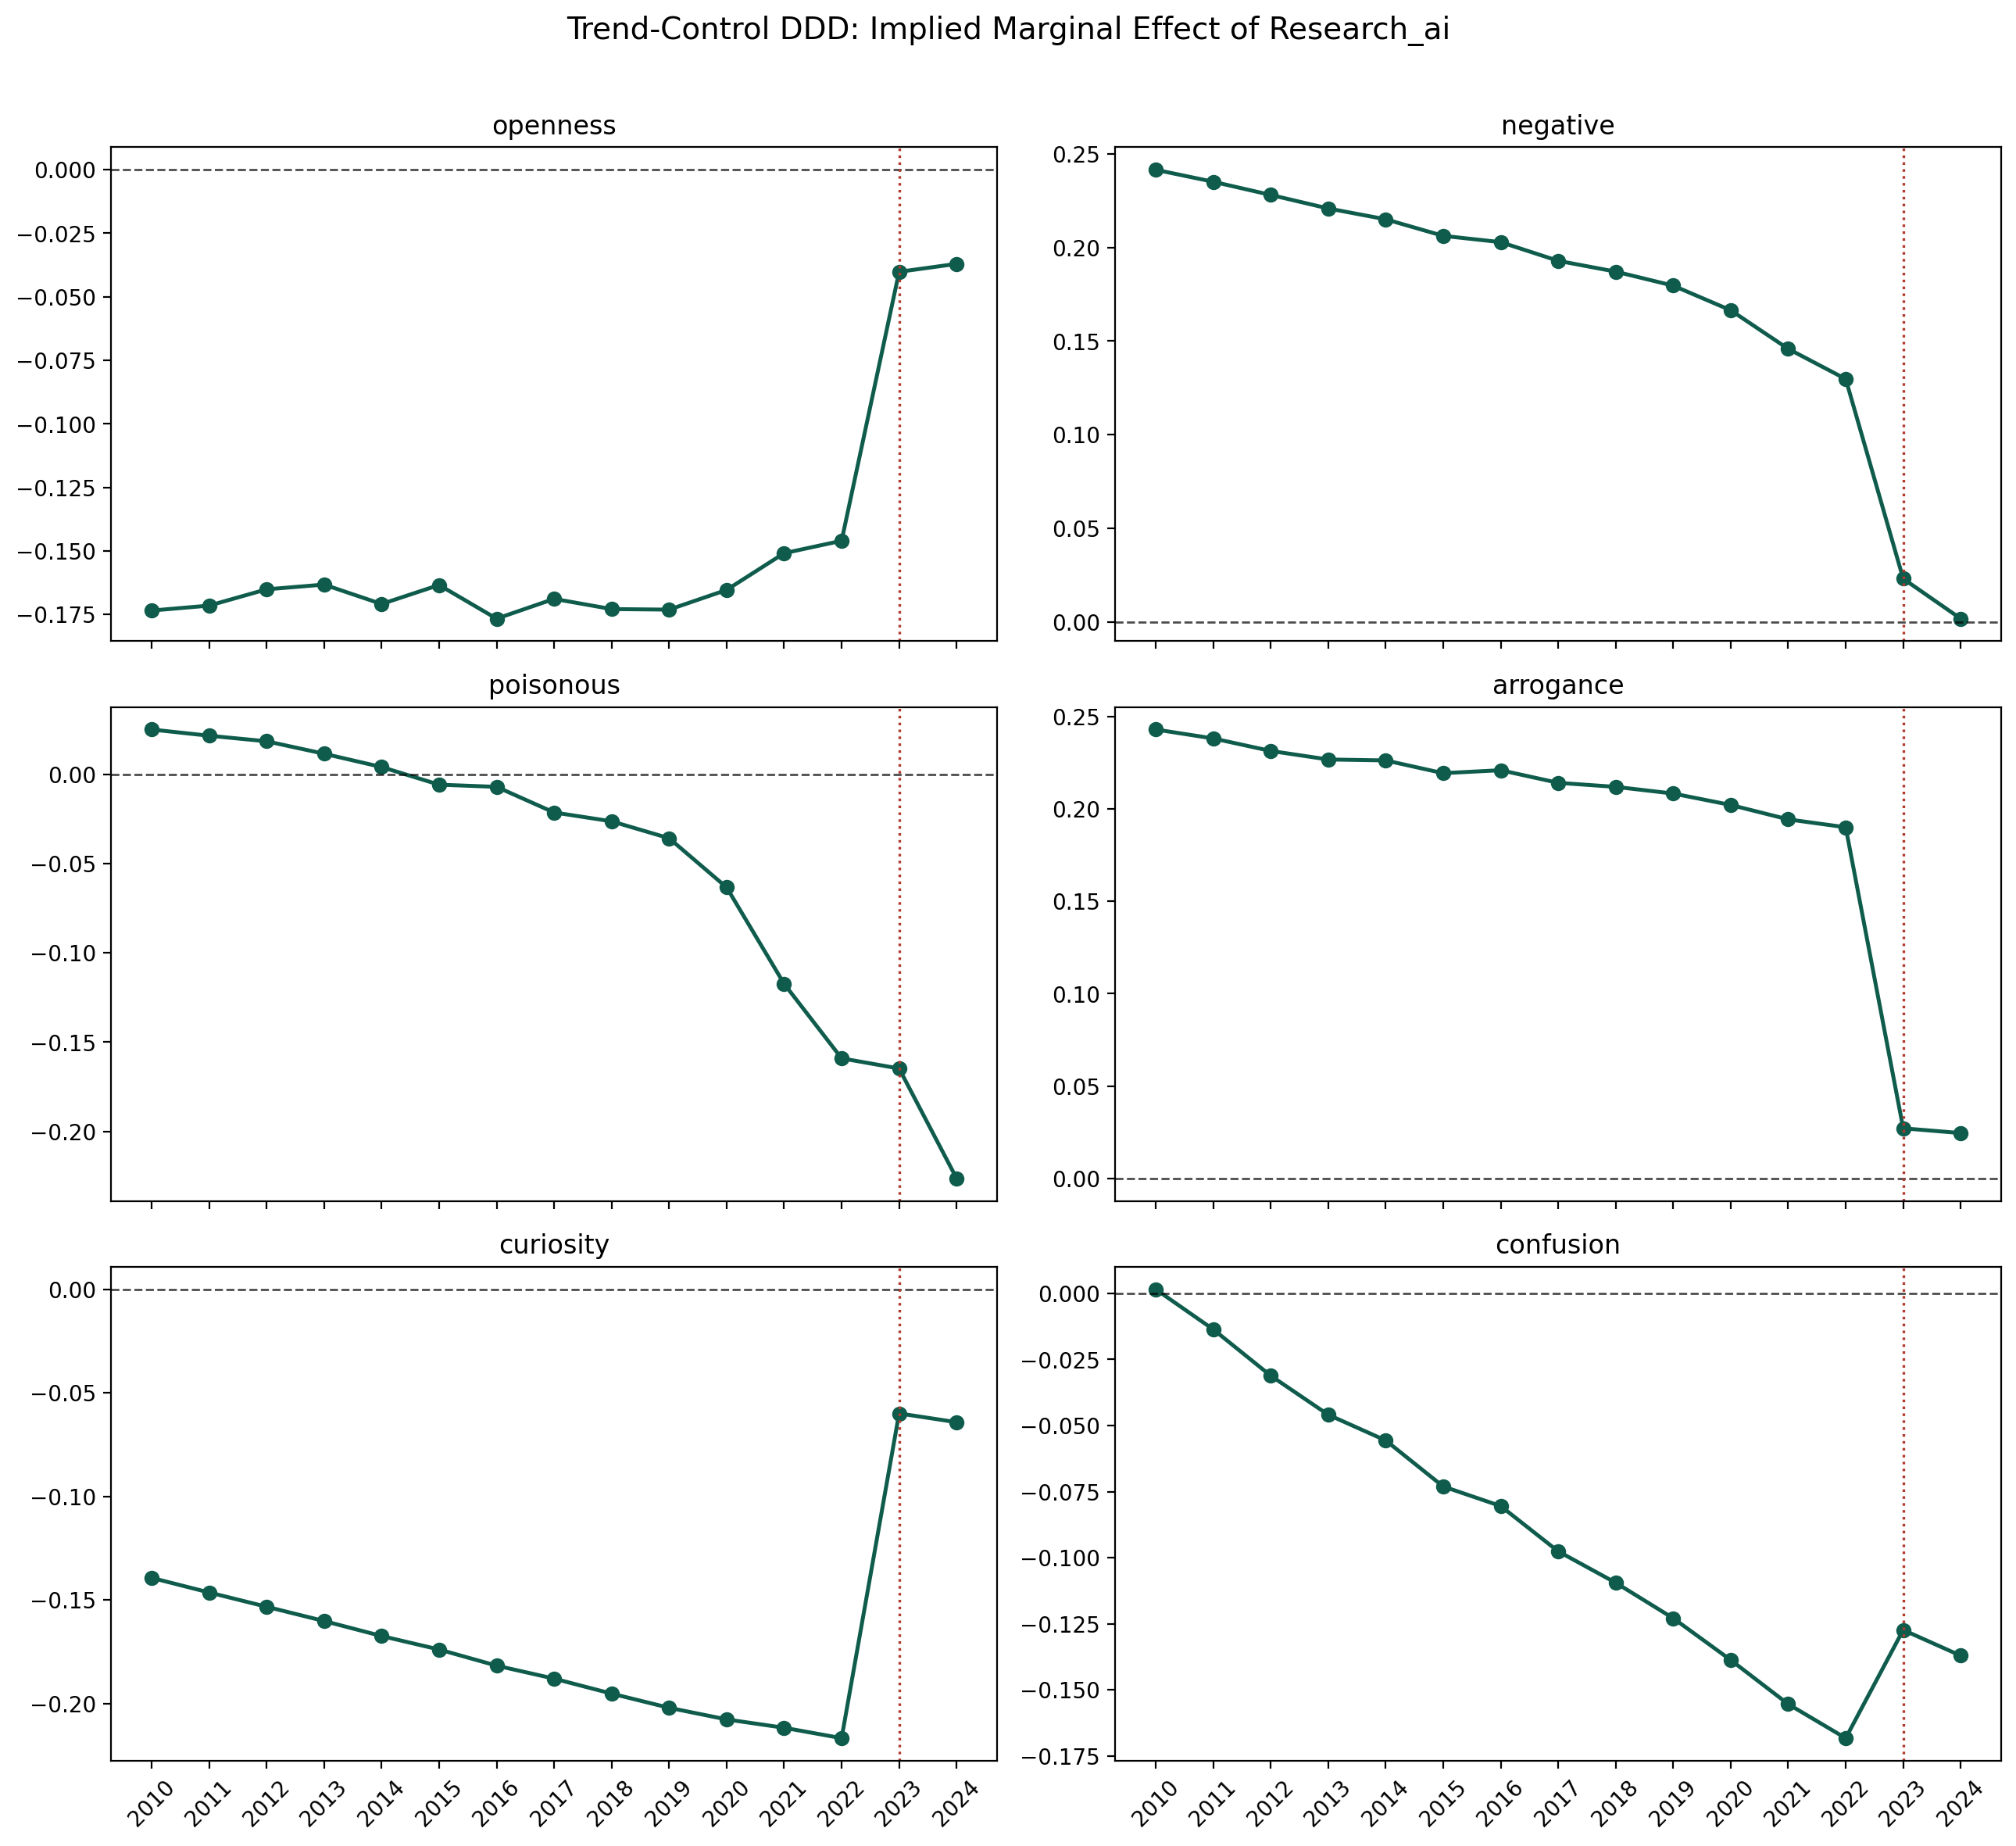
\includegraphics[width=0.95\textwidth]{photo/DDD_Trend_Break_Effects_4+.png}
    \caption{Trend-Control DDD: Implied Marginal Effect of AI\_Exposure by Year}
    \label{fig:trend_break_effects}
    {\captionsetup{justification=raggedright,singlelinecheck=false}
    \caption*{\footnotesize Notes: Each panel plots the implied marginal effect of $AI\_Exposure$ by year under the preferred trend-control DDD specification. The vertical line marks 2023.}}
\end{figure}

\FloatBarrier

\subsection{Heterogeneity Analysis}

\subsubsection{Comparison Trends}

The first heterogeneity exercise asks whether the AI pattern is special relative to alternative publication-side topic trends. We re-estimate the same DDD architecture using Platform Economics, Labor/Wages, and Gender Economics as comparison topics:

\begin{equation}
\begin{aligned}
Y_{i,t} ={}& \alpha_0 + \alpha_1 \cdot Topic_Exposure_{i,m} + \alpha_2 \cdot Topic_Trend_{m,t} + \alpha_3 \cdot AI\_Index_t \\
&+ \alpha_4 \cdot \left(Topic_Exposure_{i,m} \times Topic_Trend_{m,t}\right)
+ \alpha_5 \cdot \left(Topic_Exposure_{i,m} \times AI\_Index_t\right) \\
&+ \alpha_6 \cdot \left(Topic_Trend_{m,t} \times AI\_Index_t\right)
+ \alpha_7 \cdot \left(Topic_Exposure_{i,m} \times Topic_Trend_{m,t} \times AI\_Index_t\right)
+ X_i' \delta + \epsilon_{i,t}.
\end{aligned}
\end{equation}

These comparison trends are useful because they separate two claims that might otherwise be conflated. One claim is that AI has a distinctive pattern. A different claim is that some nearby frontier topics, especially technology-adjacent ones, may display partial similarities. The results support both ideas.

Platform Economics is the most informative comparison because it is the closest to AI in terms of digital infrastructure, online markets, and new technology adoption. It is not the same object as AI, but it belongs to the same broad family of frontier digital change. In Table \ref{tab:comparison_trends_summary}, Platform Economics shows the closest directional resemblance to AI: greater publication-side platform visibility is associated with more openness and curiosity and with less negative tone, poisonousness, and arrogance. That does not make the AI result trivial. Rather, it sharpens the interpretation that the AI pattern is linked to frontier technological change rather than to an arbitrary topic label.

Labor/Wages and Gender Economics look very different. Their topic-by-trend slopes generally move in the opposite direction from AI and from the platform comparison. This contrast matters. It means the AI result is not a generic property of any topic that becomes more visible in elite journals. The directional similarity is concentrated in the technology-adjacent benchmark, while the non-technology comparisons do not replicate the same broad softening pattern.

\begin{table}[!htbp]
    \centering
    \caption{Comparison Trends: Preferred Full DDD Specification}
    \label{tab:comparison_trends_summary}
    \footnotesize
    \setlength{\tabcolsep}{5pt}
    \renewcommand{\arraystretch}{1.0}
    \resizebox{\textwidth}{!}{%
    \begin{tabular}{lcccccc}
        \toprule
        Term & Openness & Negative tone & Poisonousness & Arrogance & Curiosity & Confusion \\
        \midrule
        Platform\_Economics\_Exposure $\times$ Platform\_Economics\_Trend & 3.3771*** & -2.7943*** & -6.6513*** & -3.6601*** & 1.0156*** & 0.0426*** \\
        Platform\_Economics\_Exposure $\times$ Platform\_Economics\_Trend $\times$ AI\_Index & -0.0029*** & -0.5122*** & -0.8080*** & -0.0985*** & -0.0837*** & -0.0905*** \\
        Labor\_Wages\_Exposure $\times$ Labor\_Wages\_Trend & -1.2594*** & 2.0695*** & 7.3091*** & 0.7226*** & -0.4198*** & 0.1879*** \\
        Labor\_Wages\_Exposure $\times$ Labor\_Wages\_Trend $\times$ AI\_Index & -0.3711*** & 0.9618*** & 2.6630*** & 0.1813*** & -0.2194*** & 0.0642*** \\
        Gender\_Economics\_Exposure $\times$ Gender\_Economics\_Trend & -0.5399*** & 0.7507*** & 0.6153*** & 0.5382*** & -0.6131*** & 0.0750*** \\
        Gender\_Economics\_Exposure $\times$ Gender\_Economics\_Trend $\times$ AI\_Index & -0.0244*** & -0.0391*** & 0.0874*** & -0.0907*** & -0.0416*** & 0.0062*** \\
        \bottomrule
    \end{tabular}}
    {\captionsetup{justification=raggedright,singlelinecheck=false}
    \caption*{\footnotesize Notes: Significance is based on year-clustered standard errors. * \(p<0.1\), ** \(p<0.05\), *** \(p<0.01\).}}
\end{table}

\FloatBarrier

\subsubsection{High-vs-Low AI Exposure}

The second heterogeneity exercise splits discussion by whether forum-side $AI\_Exposure$ is already high before the public AI wave. Let $High\_AI\_Exposure_i$ equal 1 when $AI\_Exposure_i$ is above the pre-2023 sample median. The estimating equation augments the baseline DDD with all interactions between $High\_AI\_Exposure_i$ and the AI DDD block:

\begin{equation}
\begin{aligned}
Y_{i,t} ={}& \text{Baseline DDD}_{i,t}
+ \theta_1 \cdot High\_AI\_Exposure_i
+ \theta_2 \cdot \left(AI\_Exposure_i \times High\_AI\_Exposure_i\right) \\
&+ \theta_3 \cdot \left(AI\_Trend_t \times High\_AI\_Exposure_i\right) \\
&+ \theta_4 \cdot \left(AI\_Index_t \times High\_AI\_Exposure_i\right) \\
&+ \theta_5 \cdot \left(AI\_Exposure_i \times AI\_Trend_t \times High\_AI\_Exposure_i\right) \\
&+ \theta_6 \cdot \left(AI\_Exposure_i \times AI\_Index_t \times High\_AI\_Exposure_i\right) \\
&+ \theta_7 \cdot \left(AI\_Trend_t \times AI\_Index_t \times High\_AI\_Exposure_i\right) \\
&+ \theta_8 \cdot \left(AI\_Exposure_i \times AI\_Trend_t \times AI\_Index_t \times High\_AI\_Exposure_i\right) \\
&+ X_i' \delta + \epsilon_{i,t}.
\end{aligned}
\end{equation}

Table \ref{tab:highlow_summary} reports the post-2023 AI terms for the low-exposure group together with the high-exposure differential. The first two rows should be read as the post-2023 AI pattern for relatively low-exposure discussion; the last two rows show how that pattern changes once a discussion is already strongly AI-adjacent before 2023.

Relative to the low-exposure group, the high-exposure group experiences a more favorable post-2023 adjustment for openness, negative tone, poisonousness, arrogance, and curiosity. The intuition is straightforward: discussions that were already closer to AI before the public AI wave appear to adapt more quickly once AI becomes salient at the frontier. They are not starting from the same place as the low-exposure discussions, and they do not react in the same way after 2023.

Confusion is the main exception. The high-exposure differential is positive there, suggesting that the most AI-adjacent discussions became less settled on that particular margin even as the other sentiment dimensions improved. A natural interpretation is that early AI-adjacent discussions became more technically engaged, but also more uncertain and internally contested, once frontier AI moved quickly after 2023.

\begin{table}[!htbp]
    \centering
    \caption{High-vs-Low AI Exposure Heterogeneity: Preferred Full Specification}
    \label{tab:highlow_summary}
    \footnotesize
    \setlength{\tabcolsep}{5pt}
    \renewcommand{\arraystretch}{1.0}
    \resizebox{\textwidth}{!}{%
    \begin{tabular}{lcccccc}
        \toprule
        Term & Openness & Negative tone & Poisonousness & Arrogance & Curiosity & Confusion \\
        \midrule
        Low exposure: AI\_Exposure $\times$ AI\_Index & -0.1730 & 0.2371*** & 0.3373*** & 0.2262*** & -0.1572 & -0.1261 \\
        Low exposure: AI\_Exposure $\times$ AI\_Trend $\times$ AI\_Index & -0.1962*** & -0.3579*** & -0.8521*** & 0.4329*** & -0.3037*** & -0.0748*** \\
        High-exposure differential on AI\_Exposure $\times$ AI\_Index & 0.2723** & -0.3334*** & -0.2455** & -0.4569*** & 0.3204** & 0.1719 \\
        High-exposure differential on AI\_Exposure $\times$ AI\_Trend $\times$ AI\_Index & 0.3462*** & -1.0867*** & -1.6650*** & -0.2448*** & 0.2494*** & 0.3098*** \\
        \bottomrule
    \end{tabular}}
    {\captionsetup{justification=raggedright,singlelinecheck=false}
    \caption*{\footnotesize Notes: Significance is based on year-clustered standard errors. * \(p<0.1\), ** \(p<0.05\), *** \(p<0.01\).}}
\end{table}

\FloatBarrier

\section{Robustness}
\label{sec:robustness}

\subsection{Expanded Topic-Trend Control Specification}

The first robustness check saturates the model with the full set of non-AI topic DDD blocks in addition to the AI block. Let $\mathcal{K}$ denote the set of publication-side topics with valid forum-side exposures, excluding AI itself. The estimating equation can be written as:

\begin{equation}
\begin{aligned}
Y_{i,t} ={}& \text{Baseline AI DDD}_{i,t} \\
&+ \sum_{k \in \mathcal{K}}
\Big[
\gamma_{1k} \cdot Topic_Exposure_{i,k}
+ \gamma_{2k} \cdot Topic_Trend_{k,t}
+ \gamma_{3k} \cdot \left(Topic_Exposure_{i,k} \times Topic_Trend_{k,t}\right) \\
&\hspace{2.2cm}
+ \gamma_{4k} \cdot \left(Topic_Exposure_{i,k} \times AI\_Index_t\right)
+ \gamma_{5k} \cdot \left(Topic_Trend_{k,t} \times AI\_Index_t\right) \\
&\hspace{2.2cm}
+ \gamma_{6k} \cdot \left(Topic_Exposure_{i,k} \times Topic_Trend_{k,t} \times AI\_Index_t\right)
\Big]
+ X_i' \delta + \epsilon_{i,t}.
\end{aligned}
\end{equation}

Conceptually, this matters because AI\_Trend might otherwise proxy for a broader period in which many research topics were becoming more salient at once. Table \ref{tab:all_trends_summary} shows that the AI-specific publication-trend slope remains favorable across all six outcomes even in this saturated environment. The post-2023 adjustment term is smaller and does not always move in the same direction outcome by outcome, but the core AI\_Trend slope survives intact.

\begin{table}[!htbp]
    \centering
    \caption{Expanded Topic-Trend Controls: Preferred Full Specification}
    \label{tab:all_trends_summary}
    \scriptsize
    \setlength{\tabcolsep}{4pt}
    \renewcommand{\arraystretch}{0.95}
    \resizebox{\textwidth}{!}{%
    \begin{tabular}{lcccccc}
        \toprule
        Term & Openness & Negative tone & Poisonousness & Arrogance & Curiosity & Confusion \\
        \midrule
        AI\_Exposure & -0.2074*** & 0.2015*** & 0.0791 & 0.2639*** & -0.2258*** & -0.1037*** \\
        AI\_Exposure $\times$ AI\_Trend & 3.2107*** & -4.1808*** & -16.0702*** & -3.7195*** & 0.2841*** & -2.1580*** \\
        AI\_Exposure $\times$ AI\_Index & 0.1682*** & -0.0650 & -0.0170 & -0.2589*** & 0.2363*** & 0.0328 \\
        AI\_Exposure $\times$ AI\_Trend $\times$ AI\_Index & 0.0793*** & -0.4894*** & -0.8768*** & 0.1187*** & 0.0958*** & 0.0803*** \\
        \bottomrule
    \end{tabular}}
    {\captionsetup{justification=raggedright,singlelinecheck=false}
    \caption*{\footnotesize Notes: Significance is based on year-clustered standard errors. * \(p<0.1\), ** \(p<0.05\), *** \(p<0.01\).}}
\end{table}

\FloatBarrier

\subsection{Surprise-to-Frontier Decomposition}

The second robustness check decomposes the publication-side AI\_Trend into a smooth expected component and a year-specific shock component. We define $AI\_Trend\_expected_t$ as the lagged yearly mean of $AI\_Trend_t$, and $AI\_Trend\_shock_t = AI\_Trend_t - AI\_Trend\_expected_t$.\footnote{For the first year in the sample, $AI\_Trend\_expected_t$ is set equal to the observed yearly mean.} The resulting specification is:

\begin{equation}
\begin{aligned}
Y_{i,t} ={}& \lambda_0 + \lambda_1 \cdot AI\_Exposure_i + \lambda_2 \cdot AI\_Index_t
+ \lambda_3 \cdot AI\_Trend\_expected_t + \lambda_4 \cdot AI\_Trend\_shock_t \\
&+ \lambda_5 \cdot \left(AI\_Exposure_i \times AI\_Index_t\right) \\
&+ \lambda_6 \cdot \left(AI\_Exposure_i \times AI\_Trend\_expected_t\right) \\
&+ \lambda_7 \cdot \left(AI\_Exposure_i \times AI\_Trend\_shock_t\right) \\
&+ \lambda_8 \cdot \left(AI\_Trend\_expected_t \times AI\_Index_t\right) \\
&+ \lambda_9 \cdot \left(AI\_Trend\_shock_t \times AI\_Index_t\right) \\
&+ \lambda_{10} \cdot \left(AI\_Exposure_i \times AI\_Trend\_expected_t \times AI\_Index_t\right) \\
&+ \lambda_{11} \cdot \left(AI\_Exposure_i \times AI\_Trend\_shock_t \times AI\_Index_t\right) \\
&+ X_i' \delta + \epsilon_{i,t}.
\end{aligned}
\end{equation}

This decomposition checks whether the post-2023 AI result is simply standing in for a smooth carry-forward process or whether discrete frontier jumps also matter. Table \ref{tab:surprise_frontier_summary} shows that the expected and shock components load differently across outcomes. That is precisely the value of the exercise: it indicates that the baseline AI result is not reducible to one undifferentiated trend term.

The most useful way to read the table is jointly rather than row by row. For the core valence outcomes such as openness, negative tone, poisonousness, and arrogance, the expected component typically points in the favorable direction while the shock component points the other way. That pattern suggests that gradual frontier normalization is associated with softening resistance, whereas abrupt AI jumps can trigger short-run backlash or conflict. Curiosity and confusion behave differently, which is also informative: sudden frontier jumps appear to stimulate exploratory engagement even when they create tension on the more evaluative sentiment margins.

So the surprise-to-frontier exercise should not be read as weakening the main story. Instead, it refines it. Slow-moving AI mainstreaming and abrupt AI shocks are not the same thing, and the table shows that forum-side sentiment reacts differently to those two components of frontier change.

\begin{table}[!htbp]
    \centering
    \caption{Surprise-to-Frontier Decomposition: Preferred Full Specification}
    \label{tab:surprise_frontier_summary}
    \scriptsize
    \setlength{\tabcolsep}{4pt}
    \renewcommand{\arraystretch}{0.95}
    \resizebox{\textwidth}{!}{%
    \begin{tabular}{lcccccc}
        \toprule
        Term & Openness & Negative tone & Poisonousness & Arrogance & Curiosity & Confusion \\
        \midrule
        AI\_Exposure $\times$ AI\_Index & 0.1191*** & -0.1652*** & 0.0950*** & -0.1988*** & 0.1466*** & -0.0236 \\
        AI\_Exposure $\times$ expected AI\_Trend $\times$ AI\_Index & 0.3060*** & -1.6624*** & -3.9050*** & -0.3550*** & -0.0690*** & 0.0258*** \\
        AI\_Exposure $\times$ shock AI\_Trend $\times$ AI\_Index & -0.2308*** & 2.6658*** & 8.9300*** & 0.0899*** & 0.5374*** & -0.1128*** \\
        \bottomrule
    \end{tabular}}
    {\captionsetup{justification=raggedright,singlelinecheck=false}
    \caption*{\footnotesize Notes: Significance is based on year-clustered standard errors. * \(p<0.1\), ** \(p<0.05\), *** \(p<0.01\).}}
\end{table}

\FloatBarrier

\section{Conclusions}
\label{sec:conclusion}
This paper develops TaDaS, Text as Data as Survey, and applies it to economists' reactions to AI in a setting where direct surveys are difficult to reconstruct retrospectively and may be filtered by professional self-presentation. TaDaS links elite-journal publications, which define the publication-side frontier, to EJMR discussion, which records naturally occurring professional reactions.

The empirical picture is two-sided. In the cross section, AI-related discussion is more conflictual: it is less open and less curious, and it is more negative and more arrogant than other research-related discussion. In the preferred DDD design, however, stronger publication-side AI visibility is associated with a broad softening of that resistance. The AI-specific slope on publication-side AI\_Trend is favorable for openness, negative tone, poisonousness, arrogance, curiosity, and confusion, and that conclusion survives the strengthened trend-control DDD, the comparison-trend and high-versus-low AI\_Exposure heterogeneity exercises, the saturated all-topic trend controls, and the surprise-to-frontier decomposition.

The contribution is therefore both methodological and substantive. Methodologically, TaDaS offers a portable way to turn existing text archives into structured attitude evidence. Substantively, the paper documents a profession that talks about AI with visible tension, but that tension is lower when AI is more firmly embedded in high-status research production. The evidence is descriptive rather than causal, and the mechanisms remain open: legitimacy, adaptation, and changing composition are all plausible. Those limits are important, but they do not undo the central result that publication-side AI visibility and forum-side sentiment move together in a disciplined and interpretable way.


\clearpage
\appendix

\section{Appendix: The Method of TaDaS}
\label{app:tadas_method}

\subsection{Principle and Interpretation}

Let $\mathcal{X}$ denote the text space and let
\[
\phi:\mathcal{X}\rightarrow\mathbb{S}^{d-1}\subset\mathbb{R}^d
\]
be an encoder that maps any text object to a normalized $d$-dimensional embedding. For a main-corpus observation $i$, write
\[
x_i=\phi(T_i), \qquad \|x_i\|_2=1,
\]
where $T_i$ is the observed text object. Let $y_i$ denote the outcome or score to be analyzed. A fully unrestricted linear representation of the conditional mean would take the form
\[
\mathbb{E}[y_i\mid x_i]=\alpha^\top x_i,
\qquad
\alpha\in\mathbb{R}^d .
\]
This representation is high-dimensional and difficult to interpret because the coordinates of $x_i$ are latent embedding dimensions rather than labeled social-science concepts.

TaDaS replaces the unrestricted embedding coordinates with a labeled reference system. Let the reference corpus generate $k$ topic or category vectors
\[
V=\begin{bmatrix}v_1&v_2&\cdots&v_k\end{bmatrix}\in\mathbb{R}^{d\times k},
\qquad
\|v_\ell\|_2=1 \quad \forall \ell .
\]
Each $v_\ell$ is a substantively labeled direction, such as a publication-side topic center. The corresponding TaDaS feature vector for main-corpus observation $i$ is the vector of cosine similarities
\[
s_i=s(x_i)=V^\top x_i
=
\begin{bmatrix}
v_1^\top x_i\\
\vdots\\
v_k^\top x_i
\end{bmatrix}
\in[-1,1]^k .
\]
Thus $s_{i\ell}$ measures the semantic exposure of text $i$ to labeled reference direction $\ell$.

The low-dimensional TaDaS regression is
\[
\mathbb{E}[y_i\mid s_i]=\theta^\top s_i
=\theta^\top V^\top x_i
=(V\theta)^\top x_i,
\qquad
\theta\in\mathbb{R}^k .
\]
Compared with the unrestricted model, TaDaS imposes the restriction
\[
\alpha\in\mathrm{span}(V),
\qquad
\alpha=V\theta .
\]
The estimand is therefore a $k$-dimensional parameter vector attached to labeled reference topics rather than a $d$-dimensional parameter vector attached to unnamed embedding coordinates.

The geometry of the reference system is governed by the Gram matrix
\[
G=V^\top V.
\]
If the reference directions were orthonormal, $s_i$ would be the coordinate vector of $x_i$ on the reference basis. In practice, semantic topic vectors are correlated, so $G\neq I_k$. The similarity vector $s_i=V^\top x_i$ should therefore be interpreted as a Gram-weighted coordinate representation: it records the relation between $x_i$ and each labeled reference direction without requiring those directions to be mutually orthogonal.

Equivalently, the closest point to $x_i$ in the reference span solves
\[
\widehat{\beta}_i
=
\arg\min_{\beta\in\mathbb{R}^k}\|x_i-V\beta\|_2^2 .
\]
When $G$ is nonsingular,
\[
\widehat{\beta}_i=(V^\top V)^{-1}V^\top x_i=G^{-1}s_i .
\]
TaDaS uses $s_i$ rather than $\widehat{\beta}_i$ as the empirical feature vector because cosine similarity is directly interpretable as topic exposure and remains well-defined even when topic directions are correlated or nearly collinear.

This construction gives TaDaS its cross-corpus structure. The reference matrix $V$ can be estimated from one corpus, while the observations $x_i$ and outcomes $y_i$ come from another. The two corpora need not share authors, users, journals, identifiers, or time stamps; they only need to be embedded by a common encoder $\phi$. In this paper, publication texts define $V$, EJMR texts supply $x_i$, and the resulting similarities $s_i=V^\top x_i$ enter the forum-side empirical models as survey-equivalent topic exposures. The decoder then supplies structured attitude outcomes $y_i$ for replies, but the core TaDaS mapping is the encoder-based projection from main-corpus text onto labeled reference directions.

\subsection{Main-Corpus Sample Screening}
\label{app:tadas_sample_screening}

The projection step above explains how TaDaS maps a main-corpus observation onto reference-topic directions. Before that mapping becomes useful in a regression sample, however, the main corpus must be screened so that the focal observations are compared with semantically relevant counterparts. This step follows the common-support intuition of matching designs: the researcher should not compare an interested observation with all observations in a raw archive when much of that archive lies outside the substantive support of the research question.

Let the main corpus contain normalized embeddings
\[
Z=\{z_i\}_{i=1}^N,\qquad z_i\in\mathbb{R}^d.
\]
A hierarchical clustering algorithm such as HDBSCAN produces a condensed cluster tree $\mathcal{T}$ and a set of retained leaf or branch clusters $\mathcal{C}=\{C_1,\dots,C_K\}$. Let $c(i)\in\mathcal{C}$ denote the cluster containing observation $i$. The researcher then marks a subset of clusters as focal or interested:
\[
\mathcal{F}\subset\mathcal{C},
\]
where, in this paper, $\mathcal{F}$ consists of research-related EJMR topic neighborhoods.

The key object is the local neighborhood around each focal cluster inside the hierarchy. Let $\mathrm{lca}(C,D)$ denote the lowest common ancestor of clusters $C$ and $D$ in the HDBSCAN tree, and let $\lambda(C,D)$ denote the density level at which $C$ and $D$ first merge into a common ancestor. A larger $\lambda(C,D)$ means that the two clusters meet at a denser and therefore more local part of the hierarchy. For each focal cluster $C\in\mathcal{F}$, define a set of comparable non-focal neighbors as
\[
\mathcal{M}(C)
=
\left\{
D\in\mathcal{C}\setminus\mathcal{F}:
\lambda(C,D)\geq \tau
\right\},
\]
or, equivalently in finite samples, as the $q$ nearest non-focal sibling branches under the same local ancestor:
\[
\mathcal{M}_q(C)
=
\operatorname*{arg\,topq}_{D\in\mathcal{C}\setminus\mathcal{F}}
\lambda(C,D).
\]
The screened cluster set is then
\[
\mathcal{R}
=
\mathcal{F}\cup
\bigcup_{C\in\mathcal{F}}\mathcal{M}_q(C),
\]
and the analysis sample is
\[
\mathcal{S}
=
\{i: c(i)\in\mathcal{R}\}.
\]
This rule keeps the interested topic neighborhoods and their nearest uninterested but semantically similar comparison neighborhoods. It is not a propensity-score estimator and is not presented as a causal identification device. The analogy to propensity score matching is the common-support logic: treated or interested observations should be compared to observations that are close enough to be meaningful counterparts \citep{rosenbaum1983,heckman1998matching,dehejia2002}.

The common-support condition can be written at the local branch level. For a local branch $B\subset\mathcal{C}$ that contains at least one retained focal cluster, define
\[
\pi_B
=
\frac{\sum_{i:c(i)\in B}\mathbf{1}\{c(i)\in\mathcal{F}\}}
{\sum_{i:c(i)\in B}1}.
\]
The screening rule aims to retain branches for which
\[
0<\pi_B<1,
\]
so that focal discussion and comparable non-focal discussion coexist inside the same local semantic region. Branches with $\pi_B=0$ contain no research-related focal cluster and are excluded; branches with only focal material and no nearby comparison text provide little local contrast.

This screening step also reduces measurement error. Naturally occurring forum text is sparse: many posts are short, elliptical, or only weakly informative about the research concept being measured. If the observed topic-exposure variable is written as
\[
\widetilde{s}_i=s_i+u_i,
\]
where $s_i$ is the latent semantic exposure and $u_i$ is noise from irrelevant or weakly informative text, then including distant off-topic branches raises the variance of $u_i$ and weakens the interpretation of $\widetilde{s}_i$. Under the maintained assumption that off-support branches have lower signal-to-noise for the focal research question, the screened sample satisfies
\[
\mathrm{Var}(u_i\mid i\in\mathcal{S})
<
\mathrm{Var}(u_i\mid i\in\{1,\dots,N\}),
\]
or, more cautiously, it is designed to move the analysis in that direction. The purpose of the hierarchical screen is therefore both substantive and statistical: it removes branches outside the research support and keeps the regression comparison inside a denser, more informative semantic neighborhood.

\subsection{Advantages}

The formal pieces above imply several practical advantages. Some advantages come from the reference-corpus projection, while others come from the main-corpus screening step.

\textbf{Common-support sample construction.} The hierarchical screen creates a sample with focal observations and nearby comparison observations. This improves substantive comparability and avoids estimating topic-sentiment relationships from contrasts between research discussion and semantically distant off-topic conversation.

\textbf{Noise reduction under sparse text.} Short and informal text often contains limited effective information. By excluding branches without local research support, TaDaS reduces the influence of weakly informative observations, slows the accumulation of sparsity-induced noise, and mitigates measurement error in topic-exposure variables.

\textbf{High-dimensional parameter reduction.} Directly regressing on a dense semantic vector requires estimating or reasoning about a high-dimensional coefficient whose coordinates have no stable substantive meaning. TaDaS replaces that object with a much smaller parameter vector. In the present application, $k$ is below 50, far smaller than the original embedding dimension.

\textbf{Interpretability through labeled similarities.} Each component of $\theta$ is attached to a similarity with a labeled reference direction. A coefficient on similarity to the AI topic, for example, can be interpreted as an association with AI-related semantic content rather than as an effect of an anonymous embedding coordinate.

\textbf{Corpus linking without external keys.} TaDaS can connect corpora even when they cannot be merged through shared identifiers, common authors, synchronized time units, or matched institutional units. The link is semantic rather than administrative.

\textbf{Continuous topic exposure.} Cosine-similarity variables are continuous rather than binary. Standard clustering often assigns each observation to one topic or cluster, producing a discrete classification. TaDaS instead records the degree of proximity between an observation and each reference direction. Continuous similarity measures preserve more granular semantic information and allow the empirical model to identify finer margins of association.

\textbf{Lower observer-effect bias.} Conventional survey data can be distorted by observer effects: respondents know they are being studied and may adjust their answers when the topic is sensitive. TaDaS can analyze naturally occurring text from open forums, public archives, reviews, comments, or other digital traces. When the source environment is anonymous or weakly tied to formal reputation, the resulting language may better reveal speakers' underlying psychological states, preferences, and professional tensions.

\textbf{Low-cost survey-equivalent data construction.} Rather than fielding a new questionnaire, recruiting respondents, and waiting for responses, researchers can apply an encoder-decoder workflow to publicly available text. The encoder maps text into a common semantic space, while the decoder converts relevant language into structured attitude outcomes.

For causal or quasi-causal interpretation, the framework should be read as a measurement architecture rather than as a substitute for identification. The projection $s(x)=V^\top x$ creates interpretable variables from unstructured data and summarizes the conditional mean through labeled semantic coordinates, while the empirical design determines whether coefficients on those variables can be given causal meaning. In the present application, the main contribution is to make professional discourse measurable at scale and to connect that measurement to publication-side research trends. The value of the method is precisely that the high-dimensional representation remains powerful enough to capture semantic variation, while the final empirical objects are low-dimensional, continuous, labeled, and interpretable.

\section{Sentiment Scoring Prompt}
\label{app:sentiment_prompt}

The decoder is instructed to score only the reply, to use the initiating post only as context, to anchor each dimension on a common 0--1 scale, and to return a fixed JSON schema. The full prompt template is reproduced below.

\begin{Verbatim}[fontsize=\footnotesize]
Analyze the economics dialogue and return JSON.

Task:
1. Evaluate ONLY A's attitude and affect.
2. Use Q only as contextual reference for interpreting A (do NOT score Q itself).
3. Use the bidirectional 0-1 scale below and keep explanation consistent with scores.

Global scale meaning (for every dimension):
- 0.0 = strong opposite pole
- 0.5 = no clear signal / neutral for this dimension
- 1.0 = strong presence of this dimension

Dimension anchors:
- openness:
  0.0 = strongly closed / defensive / conservative stance
  0.5 = neutral or unclear openness
  1.0 = strongly open / receptive / willing to engage
- negative:
  0.0 = clearly non-negative / positive tone
  0.5 = neither clearly positive nor negative
  1.0 = strongly negative tone
- poisonous:
  0.0 = clearly harmless / supportive
  0.5 = neither clearly toxic nor supportive
  1.0 = strongly toxic / hostile / harmful
- arrogance:
  0.0 = clearly humble / modest
  0.5 = neither clearly humble nor arrogant
  1.0 = strongly arrogant / condescending
- curiosity:
  0.0 = clearly disinterested / rejecting exploration
  0.5 = no clear curiosity signal
  1.0 = strongly curious / exploratory
- confusion:
  0.0 = clearly certain / coherent
  0.5 = neither clearly certain nor confused
  1.0 = strongly confused / disoriented

Consistency rules:
- 0.5 means "no signal", not "medium intensity".
- If A is empty or missing, return 0.5 for all six scores.
- Do not raise poisonous/negative just because Q is toxic.
- Explanation should mention how A responds to Q as context.
- Keep explanation concise.

Provided Top Topic:
{TOP_TOPIC}

Return strictly JSON with exactly these keys:
{
  "openness": 0.5,
  "negative": 0.5,
  "poisonous": 0.5,
  "arrogance": 0.5,
  "curiosity": 0.5,
  "confusion": 0.5,
  "explanation": ""
}

Q: {Q}
A: {A}
\end{Verbatim}

\section{Related Methods}
\label{app:transformer_background}

This appendix explains the transformer architecture that underlies both the encoder used for topic mapping and the decoder used for reply-level attitude scoring, followed by the clustering methods that convert encoder representations into topic centers.

\subsection{Transformer}

Transformers map a token sequence into contextual representations through repeated layers of self-attention and position-wise nonlinear transformation \citep{vaswani2017}. Let a tokenized input sequence be $t_1,\dots,t_n$. After token and position embeddings are added, the initial layer representation can be written as
\[
H^{(0)}=
\begin{bmatrix}
e(t_1)+p_1\\
\vdots\\
e(t_n)+p_n
\end{bmatrix}
\in \mathbb{R}^{n \times d},
\]
where $e(t_i)$ is the token embedding, $p_i$ is the positional embedding, and $d$ is the hidden dimension.

In one attention head, the layer state $H^{(\ell-1)}$ is linearly projected into queries, keys, and values:
\[
Q^{(\ell,h)} = H^{(\ell-1)}W_Q^{(\ell,h)}, \qquad
K^{(\ell,h)} = H^{(\ell-1)}W_K^{(\ell,h)}, \qquad
V^{(\ell,h)} = H^{(\ell-1)}W_V^{(\ell,h)},
\]
where $h$ indexes the attention head and the projection matrices have compatible dimensions. Scaled dot-product attention for that head is then
\[
\mathrm{Attn}^{(\ell,h)}(H^{(\ell-1)})
=
\mathrm{softmax}\!\left(
\frac{Q^{(\ell,h)}(K^{(\ell,h)})^\top}{\sqrt{d_k}}
\right)V^{(\ell,h)}.
\]
If there are $M$ heads, multi-head attention concatenates the head-specific outputs and applies an output projection:
\[
\mathrm{MHA}^{(\ell)}(H^{(\ell-1)})
=
\mathrm{Concat}\!\left(
\mathrm{Attn}^{(\ell,1)},\dots,\mathrm{Attn}^{(\ell,M)}
\right)W_O^{(\ell)}.
\]

Each transformer block then combines multi-head attention with a position-wise feed-forward network, residual connections, and layer normalization. A standard pre-normalization representation is
\[
\tilde{H}^{(\ell)}
=
H^{(\ell-1)} + \mathrm{MHA}^{(\ell)}\!\left(\mathrm{LN}(H^{(\ell-1)})\right),
\]
\[
H^{(\ell)}
=
\tilde{H}^{(\ell)} + \mathrm{FFN}^{(\ell)}\!\left(\mathrm{LN}(\tilde{H}^{(\ell)})\right),
\]
with
\[
\mathrm{FFN}^{(\ell)}(u)=W_2^{(\ell)}\phi\!\left(W_1^{(\ell)}u+b_1^{(\ell)}\right)+b_2^{(\ell)}.
\]
The key economic intuition for the present paper is simple: self-attention allows each token to be represented in the context of every other token in the same sequence, so the final representation is sensitive to meaning, tone, and surrounding context rather than to isolated keywords alone.

\subsection{Encoder}

Encoder models such as BERT and RoBERTa read the full input sequence bidirectionally and produce contextual representations for every token \citep{devlin2019bert,liu2019roberta}. If the final-layer encoder output for text $i$ is $H_i^{(L)} \in \mathbb{R}^{n_i \times d}$, a sentence-level embedding can be obtained through a pooling operator,
\[
x_i = \mathrm{Pool}\!\left(H_i^{(L)}\right) \in \mathbb{R}^{d}.
\]
In the present application, the encoder is not used for token prediction. It is used to place publication text and EJMR text into the same semantic geometry, so that cosine similarity and cluster structure become interpretable measures of topic proximity.

The model used for this step is All-RoBERTa Large v1 (\texttt{all-roberta-large-v1}), which combines a RoBERTa backbone with sentence-transformer style fine-tuning for semantic similarity tasks \citep{liu2019roberta,reimers2019}. That design is especially useful here because the paper needs one shared representation space that can compare short, informal forum language to formal academic titles and abstracts.

\subsection{Decoder}

Decoder models use the same transformer ingredients but impose a causal attention mask so that token $s$ can only attend to positions $1,\dots,s$ when predicting the next token. If $M \in \mathbb{R}^{n\times n}$ is the causal mask with
\[
M_{ab}=
\begin{cases}
0, & b \le a,\\
-\infty, & b>a,
\end{cases}
\]
then masked self-attention can be written as
\[
\mathrm{MaskedAttn}(H)
=
\mathrm{softmax}\!\left(
\frac{QK^\top}{\sqrt{d_k}} + M
\right)V.
\]
This architecture yields an autoregressive factorization of the output distribution:
\[
p(y_{1:T}\mid c)
=
\prod_{t=1}^{T} p(y_t \mid c, y_{1:t-1}),
\]
where $c$ denotes the conditioning context. Instruction tuning then adapts such a decoder to follow structured prompts and return useful task-specific outputs.

In this paper, the decoder is not used to generate free-form essays. It is used as a controlled scoring device. Given a prompt post $Q_j$ and a reply $A_j$, the model returns a vector of bounded attitude scores,
\[
r_j = f_{\theta}(Q_j,A_j)
=
\big(r_j^{\mathrm{open}}, r_j^{\mathrm{neg}}, r_j^{\mathrm{tox}}, r_j^{\mathrm{arr}}, r_j^{\mathrm{cur}}, r_j^{\mathrm{conf}}\big),
\]
with each component constrained to $[0,1]$ by the prompting template. The decoder used for this stage is Gemma 3 12B IT (\texttt{gemma-3-12b-it}), an instruction-tuned decoder model in the Gemma family \citep{gemmateam2025}. Relative to an encoder, its advantage here is that it can condition directly on the pair $(Q_j,A_j)$ and follow explicit scoring instructions about whose attitude is being evaluated and how the scale should be interpreted.

\subsection{UMAP}
\label{app:topic_pipeline}

Let $x_i \in \mathbb{R}^{d}$ denote the encoder representation of publication text $i$, where the text is typically a title-abstract pair embedded by the shared encoder. These vectors live in a high-dimensional semantic space. Direct clustering in that space is possible, but in practice it is often useful to first preserve the local neighborhood structure in a lower-dimensional representation. The pipeline therefore applies UMAP \citep{mcinnes2018umap} to obtain reduced vectors
\[
\tilde{x}_i = U(x_i) \in \mathbb{R}^{r},
\]
where $U(\cdot)$ denotes the fitted UMAP transformation and $r \ll d$.

The basic role of UMAP is geometric rather than supervised. It attempts to preserve nearby semantic relationships while compressing the representation to a space that is easier to cluster. In the current application, this matters because publication texts may differ in wording while still belonging to similar research areas, and the paper wants the clustering stage to operate on the local semantic structure rather than on sparse lexical overlap.

More concretely, UMAP begins by constructing a local neighborhood graph in the original embedding space. Around each publication vector $x_i$, it identifies nearby observations and converts the corresponding distances into fuzzy neighborhood weights. Let $p_{i\ell}$ denote the strength of the neighborhood relation between publication texts $i$ and $\ell$ in the original encoder space. The collection of these weights defines a fuzzy graph that approximates the local manifold structure of the publication corpus.

In a standard formulation, one first defines a local connectivity offset $\rho_i$ and scale parameter $\sigma_i$ for each point, and then writes the directed neighborhood weight from $i$ to $\ell$ as
\[
p_{\ell \mid i}
=
\exp\!\left(
-\frac{\max\{0,\|x_i-x_\ell\|-\rho_i\}}{\sigma_i}
\right).
\]
The symmetrized fuzzy weight can then be written as
\[
p_{i\ell}
=
p_{\ell \mid i}+p_{i \mid \ell}-p_{\ell \mid i}p_{i \mid \ell}.
\]
This construction allows the neighborhood scale to adapt locally rather than imposing one global radius for the entire corpus.

UMAP then searches for reduced vectors $\tilde{x}_i$ whose own low-dimensional fuzzy neighborhood graph resembles the high-dimensional one as closely as possible. If $q_{i\ell}$ denotes the corresponding neighborhood weight in the reduced space, this fitting problem can be summarized by minimizing a cross-entropy-type objective of the form
\[
\mathcal{L}_{\mathrm{UMAP}}
=
\sum_{i<\ell}
\left[
p_{i\ell}\log\!\left(\frac{p_{i\ell}}{q_{i\ell}}\right)
+ (1-p_{i\ell})\log\!\left(\frac{1-p_{i\ell}}{1-q_{i\ell}}\right)
\right].
\]

In the low-dimensional space, UMAP typically uses a smooth heavy-tailed kernel such as
\[
q_{i\ell}
=
\left(1+a\|\tilde{x}_i-\tilde{x}_\ell\|^{2b}\right)^{-1},
\]
where $a>0$ and $b>0$ govern how quickly similarity decays with distance. This choice helps preserve local neighborhoods while preventing the reduced embedding from collapsing globally.

The first term rewards keeping genuinely close publication texts near one another after reduction, while the second discourages unrelated texts from collapsing together. In intuitive terms, UMAP is not merely shrinking dimensionality for convenience. It is preserving the local semantic geometry that later allows the clustering step to identify coherent research areas rather than arbitrary clouds of points.

\subsection{HDBSCAN}

After dimensionality reduction, the reduced vectors $\tilde{x}_i$ are partitioned with HDBSCAN \citep{campello2013hdbscan,mcinnes2017hdbscan}. Let $g(i) \in \{1,\dots,K\}$ denote the cluster assignment for publication $i$, where $K$ is the resulting number of retained topic clusters. HDBSCAN is useful here because it is density-based and inherently hierarchical: it allows clusters to differ in size and shape, and it can leave some observations weakly assigned or effectively treated as noise rather than forcing every document into an equally compact partition. The hierarchy is not an auxiliary diagnostic added after clustering; it is a native output of the algorithm's density-tree construction.

Its logic can be described in three steps. First, for each point $\tilde{x}_i$, define a core distance $c_i$ that captures the radius required to reach a target local neighborhood size. If $m$ denotes the minimum neighborhood size used by the procedure, one can write
\[
c_i = d_m(\tilde{x}_i),
\]
where $d_m(\tilde{x}_i)$ is the distance from $\tilde{x}_i$ to its $m$-th nearest neighbor. Second, replace ordinary pairwise distance with mutual-reachability distance,
\[
d_{\mathrm{mr}}(i,\ell)
=
\max\{c_i,\; c_\ell,\; \|\tilde{x}_i-\tilde{x}_\ell\|\}.
\]
This transformation makes thin bridges between sparse regions less influential and turns density structure into a more stable geometric object. Third, HDBSCAN builds a minimum spanning tree using these mutual-reachability distances, interprets that tree across all density thresholds, and condenses the resulting hierarchy into a set of stable clusters.

It is often useful to switch from distance to density level by defining
\[
\lambda_{i\ell} = \frac{1}{d_{\mathrm{mr}}(i,\ell)}.
\]
As the density threshold $\lambda$ changes, connected components appear, split, and disappear. HDBSCAN therefore studies a full cluster tree indexed by density rather than selecting a partition at one fixed cutoff.

The key object is therefore not one flat partition chosen at one arbitrary distance cutoff, but a hierarchy of candidate clusters across density levels. The final cluster labels used in a regression dataset are a selected flat representation of this richer tree, while the condensed hierarchy records which topics are parents, descendants, or close local siblings. Clusters that persist across a wider range of density thresholds are treated as more stable. This persistence logic is important in the present setting because some research areas are broad and dense while others are narrower, emerging, or only weakly separated. A density-based hierarchical method is therefore better aligned with the semantic heterogeneity of both the publication corpus and the EJMR corpus than a rigid equal-variance partition would be.

Formally, if cluster $C$ is born at density level $\lambda_{\mathrm{birth}}(C)$ and observation $i \in C$ remains attached to that cluster until level $\lambda_i^{\ast}$, a generic stability score can be written as
\[
\mathrm{Stability}(C)
=
\sum_{i \in C}\left(\lambda_i^{\ast}-\lambda_{\mathrm{birth}}(C)\right).
\]
Clusters with larger stability are interpreted as more persistent density structures and are therefore retained in the condensed hierarchy.

\section{Topic Clusters}
\label{app:topic_clusters}

This appendix explains how the paper moves from clustered publication embeddings to topic keywords, topic centers, and finally the topic-similarity variables used in the EJMR-side analysis.

\subsection{Complete EJMR Cluster Hierarchy}
\label{app:ejmr_sample_screening}

Section \ref{sec:data} describes the research-oriented EJMR screening rule used to construct the analysis sample. This appendix provides the full forum-side hierarchy and additional examples behind that decision. The broader raw EJMR archive contains 7,989,637 posts, while the screened analysis sample contains 1,304,483 post-level observations.

The complete hierarchy in Figure \ref{fig:ejmr_hierarchical_overview} shows that the forum-side topic structure is much broader than the research content used in the regressions. Research-related clusters appear together with clusters about ordinary consumption, entertainment, lifestyle, and other off-topic conversation. The sample-screening rule therefore uses the HDBSCAN hierarchy to retain research-relevant local neighborhoods and their nearest comparable branches, while excluding branches that have no neighboring research topic at the local hierarchical level.

\begin{figure}[H]
    \centering
    \includegraphics[width=0.96\textwidth,height=0.82\textheight,keepaspectratio]{hierarchical_overview.png}
    \caption{Complete EJMR Topic Cluster Hierarchy}
    \label{fig:ejmr_hierarchical_overview}
\end{figure}

\begin{figure}[H]
    \centering
    \includegraphics[width=0.88\textwidth]{Post_Distribution_14years.png}
    \caption{Distribution of EJMR Posts Over Time}
    \label{fig:post_distribution}
\end{figure}

\subsection{Topic Similarity Construction}

Once clusters are obtained, the paper summarizes each cluster with representative keywords using class-based TF-IDF, following the logic used in BERTopic-style neural topic modeling \citep{grootendorst2022bertopic}. Let $\mathcal{D}_k$ denote the meta-document formed by concatenating the texts of all publications assigned to cluster $k$. For token $w$, let $f_{kw}$ denote its within-cluster frequency in $\mathcal{D}_k$, and let $n_w$ denote the number of cluster-level meta-documents in which token $w$ appears. A generic c-TF-IDF score can then be written as
\[
\omega_{kw} = \frac{f_{kw}}{\sum_{v} f_{kv}} \cdot \log\!\left(\frac{K}{n_w}\right).
\]

High values of $\omega_{kw}$ indicate tokens that are common within cluster $k$ but relatively distinctive across clusters. The reported topic keywords in the main text are drawn from the highest-scoring terms under this cluster-level weighting scheme. This is why the topic labels should be read as semantic summaries of clusters rather than as manually imposed field names.

After the publication-side clusters are formed, the pipeline returns to the original encoder space to define topic centers. For cluster $k$, let
\[
\tau_k = \frac{1}{|\mathcal{C}_k|} \sum_{i \in \mathcal{C}_k} x_i
\]
denote the mean publication embedding for that cluster, where $\mathcal{C}_k = \{i : g(i)=k\}$. The vector $\tau_k$ is the publication-side topic center used as the benchmark for topic similarity.

Now let $z_j \in \mathbb{R}^{d}$ denote the encoder representation of EJMR text $j$. The topic-similarity score between EJMR text $j$ and publication-side topic $k$ is then computed as cosine similarity:
\[
s_{jk} = \cos(z_j,\tau_k)
= \frac{z_j^\top \tau_k}{\|z_j\| \, \|\tau_k\|}.
\]

These $s_{jk}$ scores are the topic-similarity variables that later enter the empirical analysis. In words, the paper first learns publication-side topics, then summarizes each topic by the mean semantic location of the papers in that cluster, and finally measures how close each EJMR text is to those publication-side topic centers.

\subsection{Additional Topic Proxy Trends}

Figures \ref{fig:appendix_proxy_trend_2} and \ref{fig:appendix_proxy_trend_3} supplement the main-text topic-trend figure by displaying additional publication-side topic proxy series. They are constructed in the same way as Figure \ref{fig:proxy_trend}: each panel traces the annual publication-side intensity of a topic in the elite-journal corpus.

\begin{figure}[H]
    \centering
    \includegraphics[width=0.96\textwidth]{Proxy_Trend_2.png}
    \caption{Additional Publication-Side Topic Proxy Trends I}
    \label{fig:appendix_proxy_trend_2}
\end{figure}

\begin{figure}[H]
    \centering
    \includegraphics[width=0.96\textwidth]{Proxy_Trend_3.png}
    \caption{Additional Publication-Side Topic Proxy Trends II}
    \label{fig:appendix_proxy_trend_3}
\end{figure}

\subsection{Illustrative Cases}

\begingroup
\scriptsize
\setlength{\LTcapwidth}{\textwidth}
\begin{longtable}{p{0.18\textwidth}p{0.72\textwidth}}
\caption{Illustrative Publication Cases by Topic}\label{tab:paper_topic_cases}\\
\toprule
Topic & Illustrative paper titles \\
\midrule
\endfirsthead
\toprule
Topic & Illustrative paper titles \\
\midrule
\endhead
AI & \casepair{ITERATIVE ALTERNATIVE EVALUATION WITHIN HUMAN-ARTIFICIAL INTELLIGENCE PROBLEMSOLVING: AN EXTENSION TO RAISCH AND FOMINA'S ``COMBINING HUMAN AND ARTIFICIAL INTELLIGENCE''}{Algorithmic Interactions in Open Source Work} \\
Econometrics & \casepair{Post-Selection and Post-Regularization Inference in Linear Models with Many Controls and Instruments}{MACHINE LEARNING IN ECONOMETRICS Double/Debiased/Neyman Machine Learning of Treatment Effects} \\
Health Economics & \casepair{Are Drugs Substitutes or Complements for Intensive (and Expensive) Medical Treatment}{Will Public Sector Retiree Health Benefit Plans Survive? Economic and Policy Implications of Unfunded Liabilities} \\
Family Business & \casepair{Socioemotional Wealth and Proactive Stakeholder Engagement: Why Family-Controlled Firms Care More About Their Stakeholders}{When More Is Better: Multifamily Firms and Firm Performance} \\
Labor and Wages & \casepair{A firm's external environment and the hiring of a non-standard workforce: implications for organisations}{Offshoring, Transition, and Training: Evidence from Danish Matched Worker-Firm Data} \\
Gender Economics & \casepair{Sexual Harassment at Work: A Decade (Plus) of Progress}{Thinking Like a Feminist: What Feminist Theory Has to Offer Sociology} \\
Personnel Economics & \casepair{For the Want of a Nail: The Interaction of Managerial Capacity and Human Resource Management on Organizational Performance}{REFLECTIONS ON THE 2014 DECADE AWARD: IS THERE STRENGTH IN THE CONSTRUCT OF HR SYSTEM STRENGTH?} \\
Public Governance & \casepair{``We're not there to lead'': Professional roles and responsibilities in ``citizen-led'' co-production}{Putting Conflict Where It Belongs: A Response to ``Creating Shared Responsibility through Respect for Military Culture: The Russian and American Cases''} \\
Firm Strategy & \casepair{Strategic Management and Performance in Public Organizations: Findings from the Miles and Snow Framework}{A Proposal to Organize and Promote Replications} \\
Behavioral Economics & \casepair{Mutualistic Coupling Between Vocabulary and Reasoning Supports Cognitive Development During Late Adolescence and Early Adulthood}{Hunger as a Context: Food Seeking That Is Inhibited During Hunger Can Renew in the Context of Satiety} \\
Venture Capital & \casepair{(Non-)Precautionary Cash Hoarding and the Evolution of Growth Firms}{A Rift in the Ground: Theorizing the Evolution of Anchor Values in Crowdfunding Communities through the Oculus Rift Case Study} \\
Entrepreneurship & \casepair{Legitimately distinct entrepreneurial stories in evolving market categories}{Liquidity, Risk, and Occupational Choices} \\
Supply Chain Economics & \casepair{Cascades and Fluctuations in an Economy with an Endogenous Production Network}{COMPLEMENTARITY, CAPABILITIES, AND THE BOUNDARIES OF THE FIRM: THE IMPACT OF WITHIN-FIRM AND INTERFIRM EXPERTISE ON CONCURRENT SOURCING OF COMPLEMENTARY COMPONENTS} \\
Game Theory & \casepair{Carrot or Stick? The Evolution of Reciprocal Preferences in a Haystack Model}{The Law of the Few} \\
Mergers and Acquisitions & \casepair{Advancing Firm Growth Research: A Focus on Growth Mode Instead of Growth Rate}{How do US firms grow? New evidence from a growth decomposition} \\
Executive Compensation & \casepair{CEO Compensation and Board Structure Revisited}{That Could Have Been Me: Director Deaths, CEO Mortality Salience, and Corporate Prosocial Behavior} \\
Online Reviews & \casepair{IS MORE STRUCTURE REALLY BETTER? A COMPARISON OF FRAME-OF-REFERENCE TRAINING AND DESCRIPTIVELY ANCHORED RATING SCALES TO IMPROVE INTERVIEWERS' RATING QUALITY}{Evaluating Frame-of-Reference Rater Training Effectiveness Using Performance Schema Accuracy} \\
Platform Economics & \casepair{Welcome contributor or no price competitor? The competitive interaction of free and priced technologies}{Evolutionary Competition in Platform Ecosystems} \\
Innovation and Patents & \casepair{Historical Disease Prevalence, Cultural Values, and Global Innovation}{Green innovation and firms' financial and environmental performance: The roles of pollution prevention versus control} \\
International Business & \casepair{Taking root in fertile ground: Community context and the agglomeration of hybrid companies}{Location of Decision Rights Within Multinational Firms} \\
Credit Risk & \casepair{Is Age a Determinant of SMEs' Financing Decisions? Empirical Evidence Using Panel Data Models}{Franchisees and Loan Default on Third-Party Guarantee Loans: Evidence From the United States} \\
Business Ethics & \casepair{Stretching the Moral Gray Zone: Positive Affect, Moral Disengagement, and Dishonesty}{Etiquette and Effort: Holding Doors for Others} \\
Team Productivity & \casepair{Top management team role structure: A vantage point for advancing upper echelons research}{Reframing talent identification as a status-organising process: Examining talent hierarchies through data mining} \\
Advertising Economics & \casepair{Spatiotemporal Allocation of Advertising Budgets}{Advertising Effects in Presidential Elections} \\
Retail Pricing & \casepair{Demand agglomeration economies, neighbor heterogeneity, and firm survival: The effect of HHGregg's bankruptcy}{Demand agglomeration economies, neighbor heterogeneity, and firm survival: The effect of HHGregg's bankruptcy} \\
Racial Inequality & \casepair{Unraveling Complexities of Latino Racialization}{The Long-Run Effect of Mexican Immigration on Crime in US Cities: Evidence from Variation in Mexican Fertility Rates} \\
Intergenerational Mobility & \casepair{Culture and Durable Inequality}{Cash or Condition? Evidence from a Cash Transfer Experiment} \\
Risk Preferences & \casepair{Measuring Probabilistic Risk Attitudes}{Human Decision Making in Dynamic Resource Allocation} \\
Consumer Demand & \casepair{The Joint Sales Impact of Frequency Reward and Customer Tier Components of Loyalty Programs}{Lead Offer Spillovers} \\
Brand Marketing & \casepair{POLISHING THE GILT EDGE: ELITE CATEGORY ENDURANCE AND SYMBOLIC BOUNDARIES IN US LUXURY HOTELS, 1790--2015}{Consumer Reactions to Brand Extensions in a Competitive Context: Does Fit Still Matter?} \\
Hedge Funds & \casepair{The term structure and inflation uncertainty}{Monetary Policy and Rational Asset Price Bubbles} \\
Earnings Management & \casepair{Disclosure Substitution}{Tacit Collusion and Voluntary Disclosure: Theory and Evidence from the US Automotive Industry} \\
\bottomrule
\end{longtable}
\endgroup

\section{Appendix Regression Tables}



% === APPENDIX: MAIN EFFECT TABLES ===
\begin{table}[H]
    \centering
    \caption{Raw Results for Openness}
    \label{tab:openness_main_effects}
    \resizebox{\textwidth}{!}{
    \begin{tabular}{lrrrr}
        \toprule
         & (1) & (2) & (3) & (4) \\
        \midrule
        AI\_Exposure & -0.1699*** & -0.1705*** & -0.1246*** & -0.1221*** \\
         & (0.0174) & (0.0175) & (0.0176) & (0.0176) \\
        Behavioral economics & -0.1754*** & -0.1022*** & -0.1077*** & -0.0750*** \\
         & (0.0124) & (0.0125) & (0.0126) & (0.0132) \\
        Business ethics & -0.9441*** & -0.8420*** & -0.7845*** & -0.7324*** \\
         & (0.0383) & (0.0384) & (0.0384) & (0.0391) \\
        Econometrics & 0.3105*** & -0.0200 & 0.0087 & 0.0443* \\
         & (0.0222) & (0.0233) & (0.0233) & (0.0236) \\
        Gender economics & -0.7914*** & -0.7230*** & -0.7303*** & -0.7136*** \\
         & (0.0276) & (0.0277) & (0.0277) & (0.0278) \\
        Health economics & -0.3703*** & -0.3474*** & -0.3450*** & -0.3509*** \\
         & (0.0262) & (0.0263) & (0.0263) & (0.0264) \\
        Innovation and patents & -0.0027 & 0.0855*** & 0.0950*** & 0.0664** \\
         & (0.0281) & (0.0284) & (0.0284) & (0.0286) \\
        Labor and wages & 0.4641*** & 0.4744*** & 0.4649*** & 0.4645*** \\
         & (0.0390) & (0.0392) & (0.0392) & (0.0395) \\
        Online reviews & 0.5698*** & 0.5273*** & 0.5059*** & 0.4553*** \\
         & (0.0276) & (0.0277) & (0.0277) & (0.0280) \\
        Platform economics & -0.2503*** & -0.2622*** & -0.2389*** & -0.1876*** \\
         & (0.0279) & (0.0283) & (0.0283) & (0.0285) \\
        Venture capital & -0.1789*** & -0.1348*** & -0.1596*** & -0.1556*** \\
         & (0.0501) & (0.0505) & (0.0505) & (0.0508) \\
        \midrule
        Thread-title emotion controls & No & No & No & Yes \\
        Forum indicators & No & Yes & Yes & Yes \\
        Year fixed effects & No & No & Yes & Yes \\
        Observations & 1,304,483 & 1,304,483 & 1,304,483 & 1,304,483 \\
        Pseudo $R^2$ & 0.0012 & 0.0017 & 0.0021 & 0.0022 \\
        \bottomrule
    \end{tabular}}
\end{table}

\begin{table}[H]
    \centering
    \caption{Raw Results for Negative Tone}
    \label{tab:negative_main_effects}
    \resizebox{\textwidth}{!}{
    \begin{tabular}{lrrrr}
        \toprule
         & (1) & (2) & (3) & (4) \\
        \midrule
        AI\_Exposure & 0.1602*** & 0.1672*** & 0.1094*** & 0.1278*** \\
         & (0.0182) & (0.0183) & (0.0184) & (0.0184) \\
        Behavioral economics & 0.1973*** & 0.0979*** & 0.1069*** & 0.0133 \\
         & (0.0130) & (0.0132) & (0.0132) & (0.0138) \\
        Business ethics & 1.7379*** & 1.6024*** & 1.5324*** & 1.3181*** \\
         & (0.0400) & (0.0401) & (0.0401) & (0.0407) \\
        Econometrics & -0.5281*** & -0.1018*** & -0.1333*** & -0.1411*** \\
         & (0.0232) & (0.0244) & (0.0243) & (0.0247) \\
        Gender economics & 0.9201*** & 0.8408*** & 0.8421*** & 0.7872*** \\
         & (0.0286) & (0.0287) & (0.0287) & (0.0287) \\
        Health economics & 0.6465*** & 0.6042*** & 0.5988*** & 0.5333*** \\
         & (0.0275) & (0.0275) & (0.0275) & (0.0276) \\
        Innovation and patents & 0.4082*** & 0.2991*** & 0.2914*** & 0.2208*** \\
         & (0.0294) & (0.0297) & (0.0297) & (0.0300) \\
        Labor and wages & -0.1360*** & -0.1733*** & -0.1603*** & -0.3340*** \\
         & (0.0407) & (0.0409) & (0.0409) & (0.0412) \\
        Online reviews & -0.2801*** & -0.2328*** & -0.2027*** & -0.2386*** \\
         & (0.0288) & (0.0289) & (0.0289) & (0.0292) \\
        Platform economics & 0.6336*** & 0.6462*** & 0.6096*** & 0.4795*** \\
         & (0.0294) & (0.0298) & (0.0299) & (0.0301) \\
        Venture capital & -0.1825*** & -0.2343*** & -0.2042*** & -0.1263** \\
         & (0.0525) & (0.0530) & (0.0529) & (0.0532) \\
        \midrule
        Thread-title emotion controls & No & No & No & Yes \\
        Forum indicators & No & Yes & Yes & Yes \\
        Year fixed effects & No & No & Yes & Yes \\
        Observations & 1,304,483 & 1,304,483 & 1,304,483 & 1,304,483 \\
        Pseudo $R^2$ & 0.0026 & 0.0033 & 0.0039 & 0.0043 \\
        \bottomrule
    \end{tabular}}
\end{table}

\begin{table}[H]
    \centering
    \caption{Raw Results for Curiosity}
    \label{tab:curiosity_main_effects}
    \resizebox{\textwidth}{!}{
    \begin{tabular}{lrrrr}
        \toprule
         & (1) & (2) & (3) & (4) \\
        \midrule
        AI\_Exposure & -0.1860*** & -0.1878*** & -0.1605*** & -0.1601*** \\
         & (0.0173) & (0.0174) & (0.0175) & (0.0175) \\
        Behavioral economics & 0.0948*** & 0.1461*** & 0.1482*** & 0.0599*** \\
         & (0.0124) & (0.0126) & (0.0126) & (0.0132) \\
        Business ethics & -0.7157*** & -0.6527*** & -0.6164*** & -0.6385*** \\
         & (0.0384) & (0.0386) & (0.0386) & (0.0392) \\
        Econometrics & 0.3224*** & 0.0516** & 0.0826*** & 0.0437* \\
         & (0.0224) & (0.0234) & (0.0234) & (0.0237) \\
        Gender economics & -0.7950*** & -0.7285*** & -0.7372*** & -0.7536*** \\
         & (0.0280) & (0.0281) & (0.0281) & (0.0282) \\
        Health economics & -0.2098*** & -0.2100*** & -0.2142*** & -0.2130*** \\
         & (0.0263) & (0.0264) & (0.0264) & (0.0265) \\
        Innovation and patents & 0.1719*** & 0.2437*** & 0.2519*** & 0.2048*** \\
         & (0.0281) & (0.0284) & (0.0284) & (0.0287) \\
        Labor and wages & 0.2400*** & 0.2516*** & 0.2457*** & 0.2981*** \\
         & (0.0392) & (0.0394) & (0.0394) & (0.0397) \\
        Online reviews & 0.4221*** & 0.3730*** & 0.3625*** & 0.3462*** \\
         & (0.0276) & (0.0277) & (0.0277) & (0.0280) \\
        Platform economics & -0.1934*** & -0.1915*** & -0.1772*** & -0.1360*** \\
         & (0.0280) & (0.0284) & (0.0284) & (0.0286) \\
        Venture capital & -0.2062*** & -0.1780*** & -0.2038*** & -0.1887*** \\
         & (0.0503) & (0.0508) & (0.0508) & (0.0511) \\
        \midrule
        Thread-title emotion controls & No & No & No & Yes \\
        Forum indicators & No & Yes & Yes & Yes \\
        Year fixed effects & No & No & Yes & Yes \\
        Observations & 1,304,483 & 1,304,483 & 1,304,483 & 1,304,483 \\
        Pseudo $R^2$ & 0.0010 & 0.0014 & 0.0017 & 0.0018 \\
        \bottomrule
    \end{tabular}}
\end{table}

\begin{table}[H]
    \centering
    \caption{Raw Results for Poisonousness}
    \label{tab:poisonous_main_effects}
    \resizebox{\textwidth}{!}{
    \begin{tabular}{lrrrr}
        \toprule
         & (1) & (2) & (3) & (4) \\
        \midrule
        AI\_Exposure & -0.0638*** & -0.0659*** & -0.1094*** & -0.1000*** \\
         & (0.0184) & (0.0185) & (0.0186) & (0.0186) \\
        Behavioral economics & 0.3378*** & 0.2273*** & 0.2294*** & 0.2069*** \\
         & (0.0132) & (0.0134) & (0.0134) & (0.0141) \\
        Business ethics & 1.4185*** & 1.2674*** & 1.2045*** & 1.0999*** \\
         & (0.0406) & (0.0407) & (0.0407) & (0.0414) \\
        Econometrics & -0.6368*** & -0.1512*** & -0.1858*** & -0.1860*** \\
         & (0.0238) & (0.0249) & (0.0249) & (0.0252) \\
        Gender economics & 1.0232*** & 0.9457*** & 0.9467*** & 0.9273*** \\
         & (0.0290) & (0.0290) & (0.0290) & (0.0291) \\
        Health economics & 0.5442*** & 0.4949*** & 0.4949*** & 0.4648*** \\
         & (0.0279) & (0.0280) & (0.0280) & (0.0280) \\
        Innovation and patents & 0.5219*** & 0.3897*** & 0.3800*** & 0.3618*** \\
         & (0.0299) & (0.0301) & (0.0301) & (0.0304) \\
        Labor and wages & -0.4528*** & -0.4834*** & -0.4741*** & -0.5618*** \\
         & (0.0415) & (0.0416) & (0.0416) & (0.0419) \\
        Online reviews & -0.4292*** & -0.3885*** & -0.3649*** & -0.3660*** \\
         & (0.0293) & (0.0293) & (0.0293) & (0.0296) \\
        Platform economics & 0.4527*** & 0.4458*** & 0.4140*** & 0.3377*** \\
         & (0.0297) & (0.0301) & (0.0302) & (0.0304) \\
        Venture capital & -0.2695*** & -0.2959*** & -0.2583*** & -0.2072*** \\
         & (0.0532) & (0.0537) & (0.0537) & (0.0540) \\
        \midrule
        Thread-title emotion controls & No & No & No & Yes \\
        Forum indicators & No & Yes & Yes & Yes \\
        Year fixed effects & No & No & Yes & Yes \\
        Observations & 1,304,483 & 1,304,483 & 1,304,483 & 1,304,483 \\
        Pseudo $R^2$ & 0.0026 & 0.0036 & 0.0041 & 0.0043 \\
        \bottomrule
    \end{tabular}}
\end{table}

\begin{table}[H]
    \centering
    \caption{Raw Results for Arrogance}
    \label{tab:arrogance_main_effects}
    \resizebox{\textwidth}{!}{
    \begin{tabular}{lrrrr}
        \toprule
         & (1) & (2) & (3) & (4) \\
        \midrule
        AI\_Exposure & 0.1407*** & 0.1539*** & 0.1544*** & 0.1557*** \\
         & (0.0143) & (0.0144) & (0.0145) & (0.0145) \\
        Behavioral economics & -0.1612*** & -0.1839*** & -0.1940*** & -0.1401*** \\
         & (0.0103) & (0.0105) & (0.0105) & (0.0110) \\
        Business ethics & -0.1763*** & -0.2002*** & -0.2116*** & -0.1844*** \\
         & (0.0315) & (0.0317) & (0.0317) & (0.0322) \\
        Econometrics & -0.2839*** & -0.1474*** & -0.1757*** & -0.1590*** \\
         & (0.0188) & (0.0197) & (0.0197) & (0.0199) \\
        Gender economics & 0.5323*** & 0.4927*** & 0.4945*** & 0.4854*** \\
         & (0.0224) & (0.0225) & (0.0225) & (0.0225) \\
        Health economics & 0.1480*** & 0.1349*** & 0.1456*** & 0.1322*** \\
         & (0.0218) & (0.0219) & (0.0219) & (0.0220) \\
        Innovation and patents & -0.0695*** & -0.0975*** & -0.1025*** & -0.0826*** \\
         & (0.0233) & (0.0235) & (0.0235) & (0.0238) \\
        Labor and wages & -0.1584*** & -0.1679*** & -0.1639*** & -0.2165*** \\
         & (0.0326) & (0.0327) & (0.0327) & (0.0329) \\
        Online reviews & -0.1003*** & -0.0698*** & -0.0657*** & -0.0713*** \\
         & (0.0229) & (0.0229) & (0.0229) & (0.0232) \\
        Platform economics & 0.0135 & 0.0448* & 0.0318 & -0.0094 \\
         & (0.0233) & (0.0236) & (0.0236) & (0.0238) \\
        Venture capital & -0.0270 & -0.0229 & -0.0010 & -0.0182 \\
         & (0.0417) & (0.0421) & (0.0421) & (0.0423) \\
        \midrule
        Thread-title emotion controls & No & No & No & Yes \\
        Forum indicators & No & Yes & Yes & Yes \\
        Year fixed effects & No & No & Yes & Yes \\
        Observations & 1,304,483 & 1,304,483 & 1,304,483 & 1,304,483 \\
        Pseudo $R^2$ & 0.0008 & 0.0010 & 0.0011 & 0.0012 \\
        \bottomrule
    \end{tabular}}
\end{table}

\begin{table}[H]
    \centering
    \caption{Raw Results for Confusion}
    \label{tab:confusion_main_effects}
    \resizebox{\textwidth}{!}{
    \begin{tabular}{lrrrr}
        \toprule
         & (1) & (2) & (3) & (4) \\
        \midrule
        AI\_Exposure & -0.0696*** & -0.0798*** & -0.1163*** & -0.1189*** \\
         & (0.0134) & (0.0135) & (0.0136) & (0.0136) \\
        Behavioral economics & 0.2011*** & 0.1486*** & 0.1697*** & 0.2205*** \\
         & (0.0097) & (0.0098) & (0.0098) & (0.0103) \\
        Business ethics & -0.2042*** & -0.2618*** & -0.2959*** & -0.2095*** \\
         & (0.0293) & (0.0294) & (0.0295) & (0.0299) \\
        Econometrics & -0.3090*** & -0.1533*** & -0.1398*** & -0.1259*** \\
         & (0.0176) & (0.0184) & (0.0184) & (0.0187) \\
        Gender economics & 0.1015*** & 0.0791*** & 0.0720*** & 0.1066*** \\
         & (0.0199) & (0.0200) & (0.0200) & (0.0200) \\
        Health economics & 0.2261*** & 0.1999*** & 0.1852*** & 0.2160*** \\
         & (0.0202) & (0.0202) & (0.0202) & (0.0203) \\
        Innovation and patents & 0.0716*** & 0.0102 & 0.0134 & 0.0691*** \\
         & (0.0217) & (0.0218) & (0.0218) & (0.0221) \\
        Labor and wages & 0.0243 & 0.0062 & 0.0140 & 0.0621** \\
         & (0.0301) & (0.0302) & (0.0302) & (0.0304) \\
        Online reviews & -0.3112*** & -0.2971*** & -0.2726*** & -0.2305*** \\
         & (0.0215) & (0.0215) & (0.0215) & (0.0217) \\
        Platform economics & 0.1867*** & 0.1554*** & 0.1309*** & 0.1568*** \\
         & (0.0217) & (0.0220) & (0.0220) & (0.0221) \\
        Venture capital & 0.0960** & 0.0895** & 0.0754* & 0.0560 \\
         & (0.0390) & (0.0394) & (0.0394) & (0.0396) \\
        \midrule
        Thread-title emotion controls & No & No & No & Yes \\
        Forum indicators & No & Yes & Yes & Yes \\
        Year fixed effects & No & No & Yes & Yes \\
        Observations & 1,304,483 & 1,304,483 & 1,304,483 & 1,304,483 \\
        Pseudo $R^2$ & 0.0003 & 0.0004 & 0.0005 & 0.0006 \\
        \bottomrule
    \end{tabular}}
\end{table}



\section{AI Usage Statement}
\label{app:ai_usage_statement}

The authors used AI-based writing tools to assist with language polishing, including improving clarity, grammar, and presentation. The research question, empirical design, data construction, model specification, statistical analysis, interpretation of results, and all substantive conclusions are the authors' own. The authors reviewed and are responsible for the final content of the paper.

\clearpage
\bibliographystyle{plainnat}
\bibliography{OpenEcon_refs}

\end{document}
